\documentclass[12pt,a4paper]{report}

\usepackage{styles/dolgozat}

\usepackage{listings}
\usepackage{styles/cpp}
\usepackage{styles/python}
\usepackage{multirow}
\usepackage{float}

\usepackage{hyperref}

\begin{document}

\pagestyle{empty} %a címlapon ne legyen semmi=empty, azaz nincs fejléc és lábléc

% A Miskolci Egyetem címere
{\large
\begin{center}
\vglue 1truecm
\textbf{\huge\textsc{Szakdolgozat}}\\
\vglue 1truecm

\includegraphics[width=4.8truecm, height=4truecm]{images/me_logo.png}\\
\textbf{\textsc{Miskolci Egyetem}}
\end{center}}

\vglue 1.5truecm %függõleges helykihagyás

% A szakdolgozat címe, akár több sorban is
{\LARGE
\begin{center}
\textbf{Gépi játékos fejlesztése \\ a Splendor nevű játékhoz}
\end{center}}

\vspace*{2.5truecm}
% A hallgató neve, évfolyam, szak(ok), a konzulens(ek) neve
{\large
\begin{center}
\begin{tabular}{c}
\textbf{Készítette:}\\
Kollár Máté\\
Programtervező informatikus
\end{tabular}
\end{center}
\begin{center}
\begin{tabular}{c}
\textbf{Témavezető:}\\
Dr. Földvári Attila József
\end{tabular}
\end{center}}
\vfill
% Keltezés: Hely, év
{\large
\begin{center}
\textbf{\textsc{Miskolc, 2022}}
\end{center}}

\newpage

\newpage

\pagestyle{empty}

%Feladatkiiras
\begin{flushleft}
\textsc{\bfseries Miskolci Egyetem}\\
Gépészmérnöki és Informatikai Kar\\
Alkalmazott Matematikai Intézeti Tanszék\hspace*{4cm}\hfil \textbf{Szám:}
\end{flushleft}
\vskip 0.5cm
\begin{center}
\large\textsc{\bfseries Szakdolgozat Feladat}
\end{center}
\vskip 0.5cm
Kollár Máté (J004TM) Programtervező informatikus jelölt részére.\newline

\noindent\textbf{A szakdolgozat tárgyköre:} Mesterséges intelligencia\newline

\noindent\textbf{A szakdolgozat címe:} Gépi játékos fejlesztése a Splendor nevű játékhoz\newline

\noindent\textbf{A feladat részletezése:}

\medskip

\emph{A Splendor egy teljes információs absztrakt társasjáték. A játék célja, hogy megszerezzen kitüntetett lapokat. Ehhez a játékosnak "motort" kell építeni, amely segítségével folyamatosan növelni lehet a játékos számára elérhető további lapokat. A dolgozat bemutatja a játék mechanikáját. Megvizsgálja, hogy a benne szereplő kártyák költségei miből adódhattak, hogyan formálódnak a játék előrehaladtával. Kidolgozásra és bemutatásra kerülnek saját heurisztikák a gépi játékos megvalósításához, például a minimax algoritmusra építve. A játék, mint alkalmazás JavaScript programozási nyelven kerül megvalósításra, melyhez a megjelenítés HTML5 Canvas segítségével történik.}

% \emph{A Splendor egy teljes információs absztrakt társasjáték. A játék célja, hogy megszerezzen kitüntetett lapokat. Ehhez a játékosnak "motort" kell építeni, amely segítségével folyamatosan növelni lehet a játékos számára elérhető további lapokat. A dolgozat bemutatja a játék mechanikáját. Megvizsgálja, hogy a benne szereplő kártyák költségei miből adódhattak, hogyan formálódnak a játék előrehaladtával. Kidolgozásra és bemutatásra kerülnek saját heurisztikák a gépi játékos megvalósításához. A játék, mint alkalmazás JavaScript programozási nyelven kerül megvalósításra, melyhez a megjelenítés HTML5 Canvas, valamint CSS segítségével történik.}

\vfill

\noindent\textbf{Témavezető:} Dr. Földvári Attila József (egyetemi adjunktus) \newline

% \noindent\textbf{Konzulens(ek):} (akkor kötelezõ, ha a témavezetõ nem valamelyik matematikai tanszékrõl való; de persze lehet egyébként is)\newline

\noindent\textbf{A feladat kiadásának ideje:} 2021. szeptember 28.\newline

%\noindent\textbf{A feladat beadásának határideje:}

\vskip 2cm

\hbox to \hsize{\hfil{\hbox to 6cm {\dotfill}\hbox to 1cm{}}}

\hbox to \hsize{\hfil\hbox to 3cm {szakfelelős}\hbox to 2cm{}}

\newpage

\vspace*{1cm}  
\begin{center}
\large\textsc{\bfseries Eredetiségi Nyilatkozat}
\end{center}
\vspace*{2cm}  

Alulírott \textbf{Kollár Máté}; Neptun-kód: \texttt{J004TM} a Miskolci Egyetem Gépészmérnöki és Informatikai Karának végzős Programtervező informatikus szakos hallgatója ezennel büntetőjogi és fegyelmi felelősségem tudatában nyilatkozom és aláírásommal igazolom, hogy \textit{ Gépi játékos fejlesztése a Splendor nevű játékhoz}
című szakdolgozatom saját, önálló munkám; az abban hivatkozott szakirodalom
felhasználása a forráskezelés szabályai szerint történt.\\

Tudomásul veszem, hogy szakdolgozat esetén plágiumnak számít:
\begin{itemize}
\item szószerinti idézet közlése idézőjel és hivatkozás megjelölése nélkül;
\item tartalmi idézet hivatkozás megjelölése nélkül;
\item más publikált gondolatainak saját gondolatként való feltüntetése.
\end{itemize}

Alulírott kijelentem, hogy a plágium fogalmát megismertem, és tudomásul veszem, hogy
plágium esetén szakdolgozatom visszautasításra kerül.

\vspace*{3cm}

\noindent Miskolc, \hbox to 2cm{\dotfill} .év \hbox to 2cm{\dotfill} .hó \hbox to 2cm{\dotfill} .nap

\vspace*{3cm}

\hspace*{8cm}\begin{tabular}{c}
\hbox to 6cm{\dotfill}\\
Hallgató
\end{tabular}



\newpage

\noindent 1.

\begin{tabular}{cl}
&szükséges (módosítás külön lapon) \\
A szakdolgozat feladat módosítása& \\
& nem szükséges\\
&\\
\hbox to 4cm{\dotfill}&\multicolumn{1}{c}{\hbox to 5cm{\dotfill}}\\
dátum& \multicolumn{1}{c}{témavezető(k)}
\end{tabular}
\vskip1.5mm

\noindent 2. A feladat kidolgozását ellenőriztem:

\vskip1.5mm

\begin{tabular}{l@{\hspace*{4cm}}l}
témavezető (dátum, aláírás):& konzulens (dátum, aláírás):\\
\dotfill&\dotfill\\
\dotfill&\dotfill\\
\dotfill&\dotfill
\end{tabular}

\vskip1.5mm

\noindent 3. A szakdolgozat beadható:

\vskip1.5mm

\begin{tabular}{@{\hspace*{1.3cm}}c@{\hspace*{2.1cm}}c}
\hbox to 4cm{\dotfill}&\multicolumn{1}{c}{\hbox to 5cm{\dotfill}}\\
dátum& \multicolumn{1}{c}{témavezető(k)}
\end{tabular}

\vskip1.5mm

\noindent 4.
\begin{tabular}[t]{@{}l@{\hspace*{1mm}}l@{\hspace*{1mm}}l@{}}
A szakdolgozat& \hbox to 3.5cm{\dotfill} &szövegoldalt\\
              & \hbox to 3.5cm{\dotfill} &program protokollt (listát, felhasználói leírást)\\
              &\hbox to 3.5cm{\dotfill}   &elektronikus adathordozót (részletezve)\\
              &\hbox to 3.5cm{\dotfill} & \\
              &\hbox to 3.5cm{\dotfill} &egyéb mellékletet (részletezve)\\
              &\hbox to 3.5cm{\dotfill} &\\
\end{tabular}
\newline tartalmaz.

\vskip1.5mm

\begin{tabular}{@{\hspace*{1.3cm}}c@{\hspace*{2.1cm}}c}
\hbox to 4cm{\dotfill}&\multicolumn{1}{c}{\hbox to 5cm{\dotfill}}\\
dátum& \multicolumn{1}{c}{témavezető(k)}
\end{tabular}

\noindent 5.

\begin{tabular}{ll}
&bocsátható\\
A szakdolgozat bírálatra& \\
& nem bocsátható\\
\end{tabular}

\vskip1.5mm

\noindent A bíráló neve: \hbox to 8cm{\dotfill}

\vskip4mm

\begin{tabular}{@{\hspace*{1.3cm}}c@{\hspace*{2.1cm}}c}
\hbox to 4cm{\dotfill}&\multicolumn{1}{c}{\hbox to 5cm{\dotfill}}\\
dátum& \multicolumn{1}{c}{szakfelelős}
\end{tabular}

\noindent 6.
\begin{tabular}[t]{@{}l@{\hspace*{1mm}}l@{\hspace*{1mm}}l@{}}
A szakdolgozat osztályzata& &\\
&a témavezető javaslata:& \hbox to 3cm{\dotfill}\\
&a bíráló javaslata:& \hbox to 3cm{\dotfill}\\
&a szakdolgozat végleges eredménye:& \hbox to 3cm{\dotfill}
\end{tabular}

\vspace*{4mm}

\noindent Miskolc, \hbox to 4.5cm{\dotfill} \hspace*{2.5cm}
\begin{tabular}[t]{cc}
\hbox to 6cm{\dotfill}\\
a Záróvizsga Bizottság Elnöke
\end{tabular}


\cleardoublepage
\pagenumbering{gobble}
\tableofcontents
\cleardoublepage
\pagenumbering{arabic}

\newpage

\pagestyle{fancy}

\Chapter{Bevezetés}

A szakdolgozatom a Splendor elnevezésű társasjáték általam módosított verziójának szoftveres megvalósításáról, a játékon belül található mesterséges intelligenciáról, valamint az ehhez kapcsolódó vizsgálatokról szól. Azért választottam ezt a témát, mert a társasjátékok világa mindig is közel állt hozzám, ezenfelül pedig a mesterséges intelligenciák köre is hasonló módon foglalkoztatott. Ennek a két területnek az ötvözésével egyértelművé vált számomra, hogy egy társasjátékkal foglalkozó dolgozatot szeretnék elkészíteni, valamint kutatásokat elvégezni azzal kapcsolatosan, hogy hogyan érdemes megvalósítani egy intelligenciát, hogy az a lehető leghatékonyabb legyen.

A második fejezetben bemutatásra kerül maga a társasjáték és a különböző fizikális és szoftveres változatai. A Splendor szabályrendszerét ismertetem a különböző játékelemek és az őket behatároló szabályok kifejtésével. Ezek mellett szerepel az általam elkészített változat szabályrendszere, a játékelemekben való eltérések.

A harmadik fejezetben a játék matematikai modelljét mutatom be, amely során kitérek a társas logikai hátterére és egy folyamatábra segítségével szemléltetem a játék folyamatának felépítését.

A negyedik fejezet az általam szoftveresen megvalósított játékról szól. Prezentálom, hogy a kezdeti terveimhez képest a játék mely részei módosultak a megvalósítás során, valamint a különböző játékelemek, szabályok és grafikai megvalósítások kivitelezését is részletezem. Ezenfelül a játék osztálydiagramját is bemutatom.

Az ötödik fejezetben az általam megvalósított öt mesterséges intelligencia kerül bemutatásra. Ismertetem a működésüket, felépítésüket, valamint mindegyik algoritmushoz bemutatom a folyamatábrát is (amelyek a függelékben tekinthetők meg). Egy táblázattal is demonstrálom a logikák funkcióinak összehasonlítását.

A hatodik fejezet a bemutatott öt mesterséges intelligenciával kapcsolatos szimulációkat tartalmazza. Ebben a részben különféle méréseket végzek annak érdekében, hogy megvizsgáljuk, hogy miként változik a játszmák felépítése a különböző algoritmusok egymás ellen való játéka során. Továbbá részletezem, hogy miként módosítottam a logikák működését az korábban elkészítettekhez képest, valamint, hogy ezeknek a módosításoknak milyen hatása volt a hatékonyságukra. Összegzésképpen pedig két táblázattal szemléltetem a különböző AI-ok egymással szembeni hatékonyságát.
\Chapter{A Splendor játék}

A Splendor társasjáték alapvetően egy reneszánsz korabeli gazdag kereskedő szerepébe helyezi a játékost \cite{rulebook}.
Forrásait felhasználva bányákat, szállítási útvonalakat szerezhet meg, kézműveseket
alkalmazhat, hogy a nyers drágaköveiből gyönyörű ékszereket készíthessen el.
A következőkben részletesen bemutatásra kerül a játék szabályrendszere, változatai és különféle megvalósításai.

\Section{Szabályrendszer}

A játék összesen negyven darab zsetont tartalmaz. A zsetonok a zöld smaragdból, a fehér gyémántból, a kék zafírból, a fekete ónixból, a piros rubinból és a sárga aranyból (joker) állnak. Mindegyik típusú zsetonból hét darabot tartalmaz a játék, kivéve az aranyból, amelyből csak ötöt. E mellett összesen kilencven kártya található a dobozban, amelyből negyven darab az első szintű, harminc a második szintű és húsz a harmadik szintű kártyapaklit, az utolsó tíz darab pedig a nemeseket ábrázoló lapokat teszi ki.

A játék előkészítése során a különböző szintű fejlődéskártya paklikat külön-külön kell megkeverni és elhelyezni a játékterület bal oldalán, oszlopot képezve alulról felfelé növekvő szintű paklik formájában.
Ezután minden pakliból, képpel felfelé négy lapot a pakli mellé, sorban
egymást követve kell letenni.
A nemeseket tartalmazó lapokat is meg kell keverni, és a játékosok számától egy darabbal több lapot kell a kártyaalakzat fölé helyezni. A megmaradt lapok a játék dobozába kerülnek vissza, azok már nem lesznek
felhasználva a játék folyamán. Végül a zsetonokat szín szerint halmokba rendezve kell lerakni.

\SubSection{Fejlődéskártyák}

Tekintély pontok megszerzéséhez a játékosoknak fejlődéskártyákat kell vásárolniuk. Ezek a kártyák a játéktér közepén találhatóak és bármelyik játékos számára megvásárolhatók a saját körükben a játék folyamán. A kézben tartott fejlődéskártyák a játékos részére tartalékot képeznek, és csak az vásárolhatja meg őket, akinek a kezében vannak.

\SubSection{A nemesek kártyalapjai}

A lapok a játék folyamán szintén a játéktéren találhatóak meg. Minden nemesi lap három tekintély pontot jelent, azonban egy játékos a saját körében csak egy nemest fogadhat.

\SubSection{Játékszabályok}

A legfiatalabb játékos kezdi a fordulót, majd a játék az óramutató járásának megfelelő irányban halad tovább.

Saját körében a játékos egyetlen cselekvést hajt végre az alábbi négy lehetőség közül:
\begin{enumerate}
	\item Elvesz három különböző színű zsetont az ékkő halmokból.
	\item Elvesz két azonos színű zsetont egy ékkő halomból (ez
	azonban csak akkor lehetséges, ha legalább négy zseton van
	abban a halomban, amikor a játékos elveszi őket).
	\item Tartalékol egy fejlődéskártyát és ezzel szerez egy arany joker zsetont.
	\item Megvásárol a középen képpel felfelé található vagy a
	saját kezében lévő tartalék fejlődéskártyák közül egyet.
\end{enumerate}

\SubSection{A zsetonok kiválasztása}

A játékos birtokában sohasem lehet tíz zsetonnál több a köre végén (beleértve a joker zsetonokat is). Amennyiben ez megtörténik, akkor annyi zsetont kell visszatenni a halmokba, hogy összesen tíz zseton maradjon a birtokában. A játékos az összes zsetont vagy annak egy részét visszateheti, amikor megszerezte őket. A játékosok birtokában lévő zsetonokat a többi játékos számára láthatóan (számolhatóan) kell tartani. 

\SubSection{Fejlődéskártyák tartalékolása}

Amennyiben a játékos tartalékolni szeretne egy fejlődéskártyát, abban az esetben felvesz egyet a játéktér közepén található kártyák közül, vagy (ha szerencsésnek érzi magát) az egyik pakli legfelső lapját veszi fel anélkül, hogy megmutatná azt a többi játékosnak. A tartalék kártyákat kézben kell tartani és nem lehet őket eldobni. Egy játékos kezében legfeljebb három ilyen kártya lehet. Csak abban az esetben játszhatók ki a játékos kezéből, ha megvásárolja azt. Tartalék kártya képzése az egyetlen módja az arany joker zseton megszerzésének. Ha már nincs elérhető, abban az esetben is tartalékolhat kártyát, de nem kap joker zsetont ezért a cselekvéséért.

\SubSection{Fejlődéskártyák megvásárlása}

Egy kártya megvásárlásához a játékosnak a kártyán látható mennyiségű zsetont el kell költenie. A joker zseton bármilyen zsetont helyettesíthet. Az elköltött zsetonok a játéktéren lévő halmokba kerülnek vissza (az arany joker is). A játékos megvásárolhat egy kártyát a játéktér közepén lévőkből vagy a korábbi körben/körökben megszerzett és kezében tartott tartalékból/tartalékokból. A kártyák által biztosított bónuszok és tekintély pontok mindenkor láthatók/számolhatók kell, hogy legyenek.

Amikor a játéktér közepéről egy kártya megvásárlásra került (akár tartaléknak, akár nem), helyette azonnal az adott szintű pakliból képpel felfelé egy másikat kell letenni. Az egész játék folyamán folyamatosan minden szintű pakliból négy képpel felfelé fordított kártyának kell középen lennie (kivéve, ha elfogytak az adott szintű pakli kártyái; ebben az esetben az üressé vált hely üres marad).

\SubSection{A bónuszok}

A korábban megvásárolt fejlődéskártyák bónuszai lehetővé teszik a következő körökben új fejlődéskártyák kevesebb költségen történő megvásárlását. A kártyákon található bónusz színe egyenértékű ugyanazon szín egy zsetonjával. Tehát, a két kék bónusszal rendelkező játékosnak amennyiben a megvásárolni kívánt kártya értéke két kék és egy zöld zseton, csak egy zöld zsetont kell megfizetnie. Amennyiben a játékosnak elegendő mennyiségű bónusz áll rendelkezésére, akkor akár ingyen is vásárolhat fejlődéskártyát.

\SubSection{A nemesek}

A játékos a köre végén ellenőrzi, hogy rendelkezik-e elegendő bónusszal, hogy a kirakott nemesek lapkái közül egynek fogadhassa látogatását. Csak az a játékos fogadhatja egy nemes látogatását, aki rendelkezik a megfelelő mennyiségű és színű bónusszal. A nemes (vagy nemesek) látogatását nem lehet visszautasítani. A nemes látogatásának fogadása nem számít cselekvésnek. Amennyiben a játékos rendelkezésére álló bónuszok lehetővé tennék több nemes látogatásának fogadását is, a játékos kiválasztja, hogy melyik látogatását fogadja. Az így megszerzett nemes lapkáját a játékos képpel felfelé maga elé helyezi.

\SubSection{A játék vége}

Amikor egy játékos megszerzi a 15. tekintély pontját véget ér a játék. Az adott fordulóban mindenki befejezheti a körét (végrehajthatja egy cselekvését), majd a tekintély pontok megszámolása után a legtöbb ponttal rendelkező játékos a nyertes. Azonos pontszám esetében az nyer, aki ezt kevesebb fejlődéskártyából érte el.

\Section{Változatok}

Az alapjátékot kettőtől négy főig lehet játszani, de a játékosok számától eltérők a zsetonok és a nemes lapkák száma. Kettő játékos esetén az arany zsetonokon kívül mindegyik típusú zsetonból csak négy darab lehet a halmokban a játék indulásakor. A nemes lapkák száma pedig három lesz. Három játékos esetén hasonlóan változnak a szabályok, annyi eltéréssel, hogy a zsetonhalmok mindegyike öt darabot fog ez esetben tartalmazni és négy nemes lapka lesz elérhető a játék során. Maximális játékosszám mellett a készletben lévő összes zseton a játéktérre kerül, a nemes lapkákból pedig öt darab lesz játékban.

\SubSection{Kiegészítők}

A játékhoz készítettek háromféle kiegészítőt is angol nyelven.

A \textit{The Cities} nevezetű kiegészítő a nemes lapkákat cseréli le város kártyákra. Ezek közül, ha az egyik játékos valamelyik város zsetonkövetelményeit eléri, felveheti azt és megkapja a rajta lévő pontszámot. A másik játékosnak ilyenkor egy köre marad arra, hogy egy másik városra összegyűjtse a szükséges zsetonokat és megvegye, így megkapja az adott város kártyát és a rajta lévő pontot \cite{cities}.

A \textit{The Strongholds} nevet viselő kiegészítő során erődítményekkel bővül az alapjáték. Ezeket az erődöket kártyákra lehet elhelyezni, hogy lefoglalja magának a játékos az adott lapot. Az erődöket más játékosok a körükben lerombolhatják annak érdekében, hogy megakadályozzák a haladást. Ha egy játékos három erődöt helyez egy kártyára, ingyenesen megvásárolhatja azt \cite{strongholds}.

Végezetül pedig a \textit{The Trading Posts} néven futó kiegészítő egy kereskedelmi vonalat fűz a játékmenetbe. Tartalmaz ugyanis egy kereskedő modult, ahol a feltüntetett követelmények teljesítésekor az ahhoz tartozó, különleges képességgel ruházza fel az adott játékost. Ilyen például az, hogy a két azonos színű zsetonfelvétel esetén kiválaszthat egy harmadik, eltérő színű zsetont is, amit felvehet az előző kettővel együtt \cite{trading}.

\SubSection{A saját változatom}

Az általam megvalósított verzió szabályrendszere eltér az alapverziótól. Az elkészített programomban az egy vagy két játékos alternatíva került implementálásra. Van lehetőség a számítógépes logika ellen játszani, és arra is, hogy két emberi játékos tudja összemérni a tudását lokálisan. Emellett az én játékverziómban a fix két játékos (akár ember, akár számítógép) ellenére mindig öt zseton van mindegyik színből a játék indulásakor, az arany zseton pedig nincs megvalósítva, és így kártyát sem lehet az adott játékosnak lefoglalni. Továbbá, a nemes lapok sincsenek jelen a játék során, csupán a kártyákon lévő pontokból lehet elérni a játék végét jelentő pontszámot. A következő módosításom, hogy a játék az alapverzióval ellentétben rögtön véget ér, ahogy az egyik játékos eléri vagy túllépi a tizenöt pontot, viszont kiegyenlítve a játékosok esélyeit, randomizáltam a kezdő játékos kijelölését. Az alapverzióban feltüntetett egy játékosnál lévő maximális zsetonokra vonatkozó szabályok sincsenek implementálva, így akármennyi zsetont felvehetnek a játékosok, nem kell visszatenniük, ha átlépik a tízet. Ritkán fordulhat elő, de bekövetkezhet, hogy a felvehető zsetonok elfogynak, és a játékos sem tud megvásárolni egy lapot sem. Ezt az eshetőséget olyan módon kezeltem, hogy a játékosok számára megjelenik egy felirat ezen állapot ismertetéséről, majd pedig ebből az üzenetből kilépve újraindul a játék. Ezt a problémát mérsékeli a korábban említett változtatásom, hogy a zsetonok számát színenként négy helyett ötre emeltem. 

\Section{Fizikális implementációk}

Fizikális megvalósítása is létezik természetesen ennek a társasjátéknak. Az első kiadást 2014-ben adták ki és jelölték az év társasjátéka díjára is, amit végül nem nyert meg (\ref{fig:physical}. ábra). A doboz a szépen megrajzolt zsetonokat, különböző szintű kártyákat és nemes lapkákat tartalmazza. 2017-ben megjelent egy vizuális újragondolással az új verziója is.

A játék fizikálisan csak az alapverziójában vásárolható meg egyedül magyarul. A kiegészítők közül is csak a \textit{The Cities} érhető el jelenleg angol nyelven.

\begin{figure}[h]
	\centering
	$\vcenter{\hbox{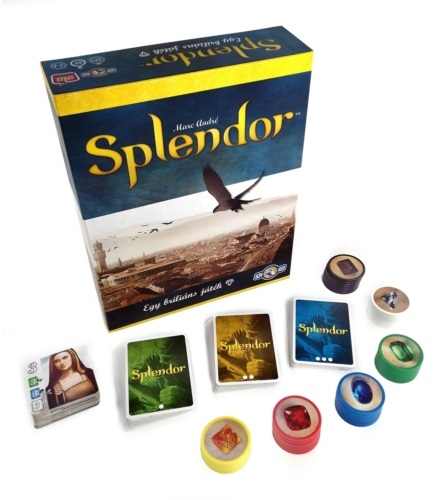
\includegraphics[width=7cm]{images/physical_edition1.jpg}}}$
	\hspace{1cm}
	$\vcenter{\hbox{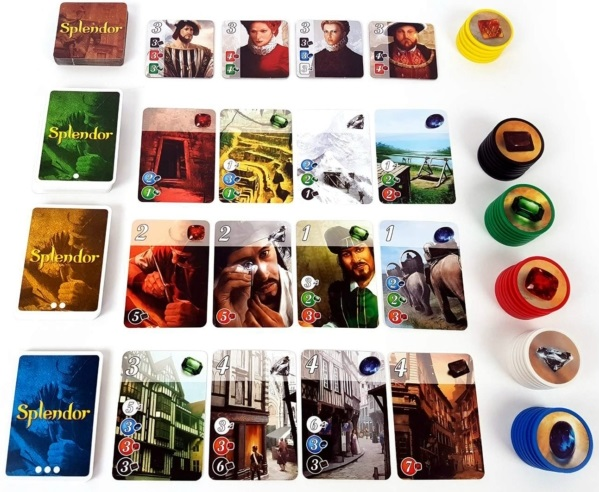
\includegraphics[width=7cm]{images/physical_edition2.jpg}}}$
	\caption{A játék fizikális megvalósítása.}
	\label{fig:physical}
\end{figure}

\Section{Szoftveres implementációk}

A szoftveres megvalósítása is elkészült a játéknak egy évvel a megjelenése után (\ref{fig:digital}. ábra). Steam-en elérhető a kiegészítőivel együtt, természetesen a játék és a kiegészítők megvásárlásával. Korábban telefonokra is elérhető volt, de ma már sajnos nem.

\begin{figure}[h]
	\centering
	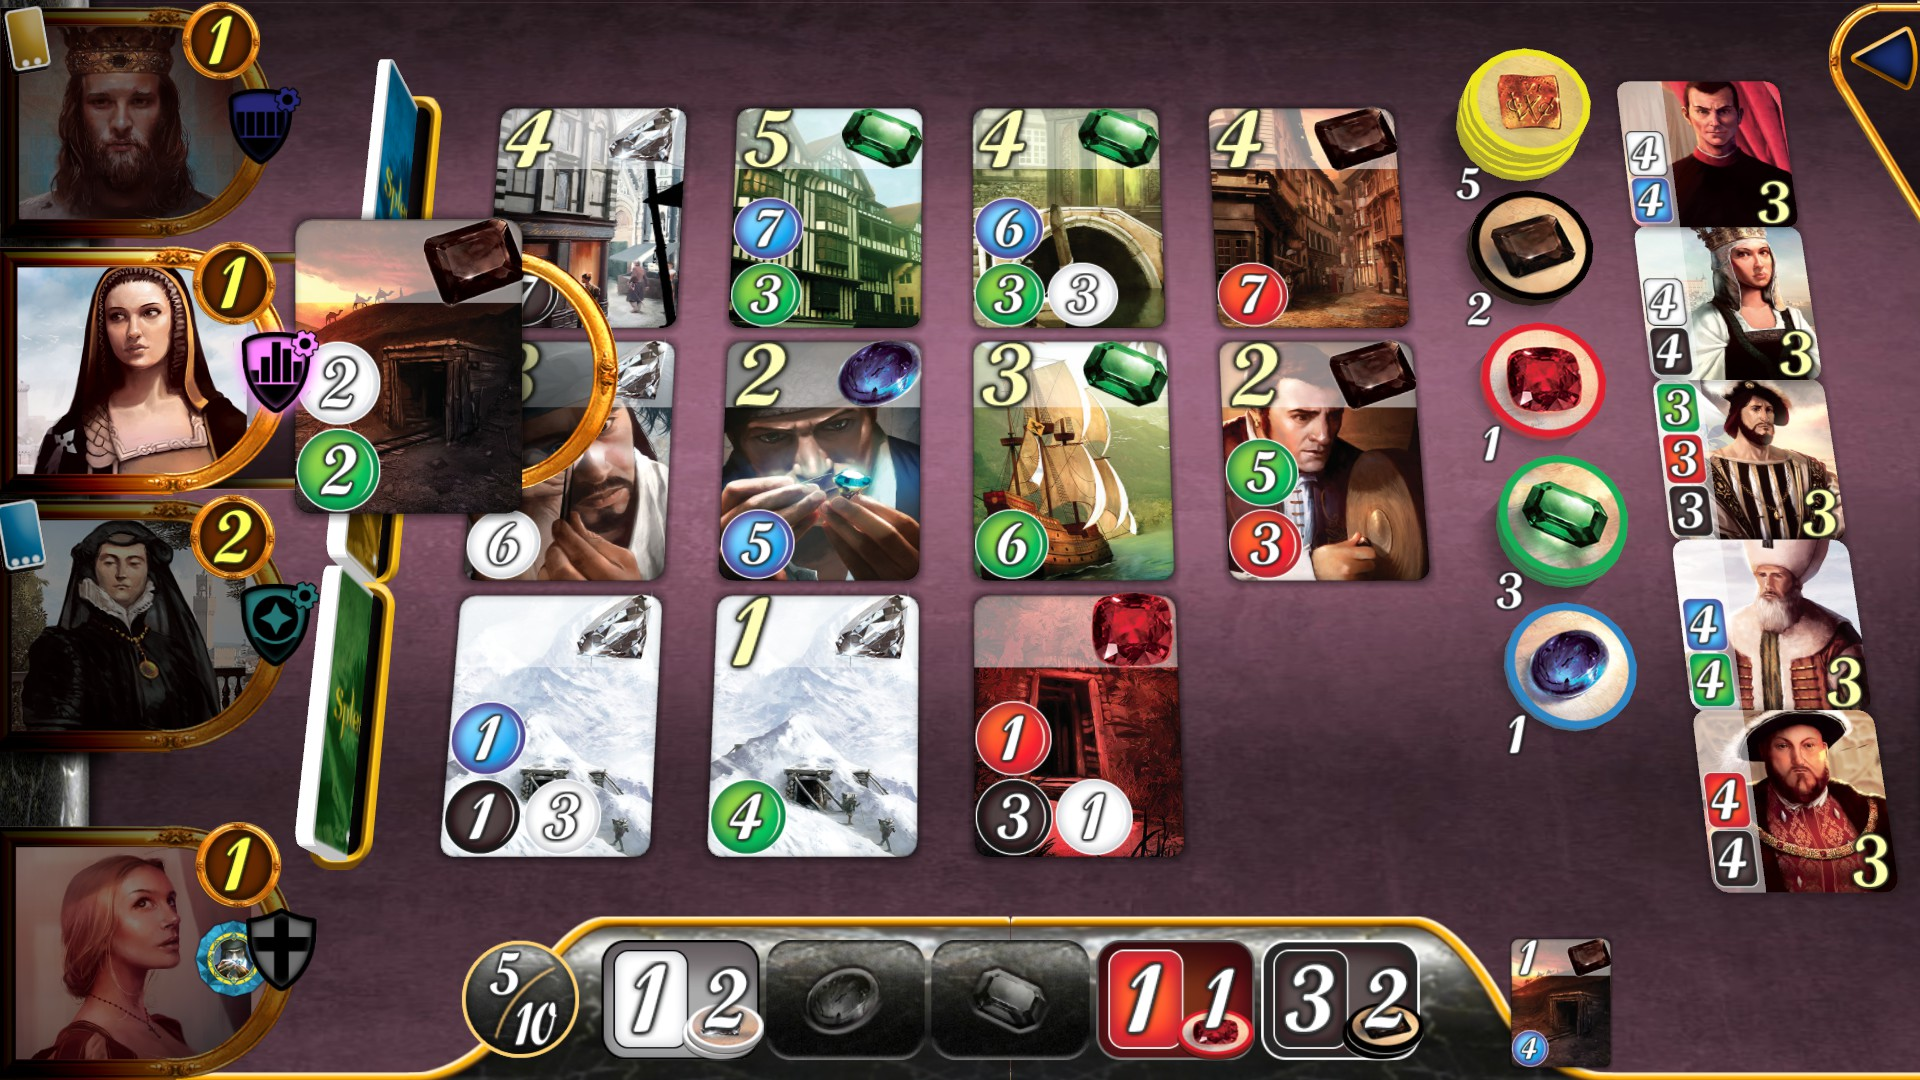
\includegraphics[scale=0.2]{images/digital_edition.jpg}
	\caption{A játék egy elérhető szoftveres megvalósítása.}
	\label{fig:digital}
\end{figure}
\Chapter{A játék matematikai modellje}

A játék véletlentől függő elemeket tartalmaz, viszont a játékosokra nézve teljes információs. A játék menete véges állapotgéppel modellezhető. A leszűkített szabályrendszerre vonatkozó játékmenetet \aref{fig:flowchart}. ábra mutatja be.

\begin{figure}[h]
\centering
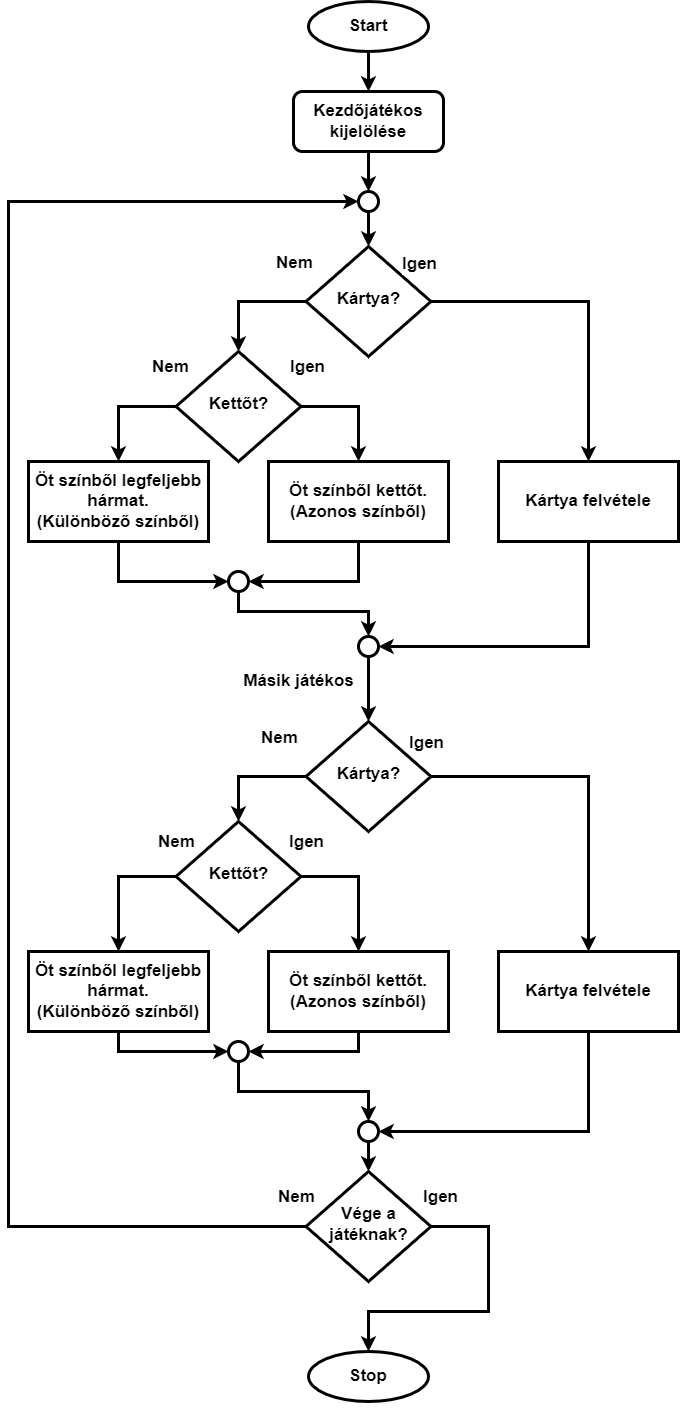
\includegraphics[scale=0.42]{images/flowchart.png}
\caption{A játék folyamatábrája.}
\label{fig:flowchart}
\end{figure}

Ahogy a folyamatábrán is látható a játék köreinek felépítése viszonylag egyszerűen zajlik. Kezdetben kijelöljük az éppen soron következő játékost, majd megkezdődik a köre. Először eldönti, hogy kártyát vagy zsetont szeretne választani az adott körben. Ha kártyát, akkor a kártyahúzás után vége a körének. Ha viszont zsetont, akkor két lehetőség áll a rendelkezésére: vagy hármat választ, egyet-egyet a különböző színekből, vagy pedig kettőt, de azonos színből. A két lehetőség valamelyikének végrehajtása után szintén átadja a kört a másik játékos számára, akinek ugyanezek a lehetőségek állnak a rendelkezésére. A második játékos köre végén megvizsgáljuk, hogy megvalósult-e a játék végét jelentő feltétel. Ha nem, akkor az első játékos köre kezdődik meg újra, és halad a folyamat a leírtak szerint, ha pedig igen, akkor a játék befejeződik.

A játékos természetesen csak a számára elérhető kártyákból és zsetonokból választhat. Egy zseton akkor elérhető a számára, ha abból legalább egy van a játéktéren, a kártya pedig akkor, ha a megvásárlásához szükséges zsetonok a birtokában vannak. Ezek a zsetonok lehetnek sima, korábban elvett zsetonok, vagy akár a kártyák korábbi megvásárlása nyomán megszerzett bónusz értékek.

A kártyalapok a játéktérre való elhelyezése randomizálva történik az adott szintű kártyapaklikból megfelelően. A kártyák szimmetrikusan szerepelnek a paklikban, így a zsetonok teljesen egyenértékűek a teljes kártyakészletet tekintve. A játék előrehaladtával és a kártyalapok fogyásával értelemszerűen folyamatosan változik ez az arány. A zsetonok értékei a játéktéren lent lévő lapok függvényében változnak. Emellett az is változtatja a zsetonok felhúzásában való lehetőségeink számát, hogy a korábbi körökben miként alakul a lent lévő zsetonok száma, mivel kettőt egy színből csak akkor lehet húzni, ha ott legalább négy van a kör kezdetekor, ezen felül pedig csak azokból a színekből lehet választani, ahol van legalább egy zseton. A játék vége felé haladva a zsetonfelhúzás kissé értékét veszti, hiszen a kártyalapok ingyen megszerzése és ezáltal a mechanizmus építése nagyobb előnyökhöz juttatja a játékosokat.

\Chapter{Az alkalmazás tervei, megvalósítása}

\Section{Képernyő szerkezet}

\SubSection{Tervek}

Kezdetben összeállítottam egy tervet, arra, hogy nagyvonalakban hogyan is képzelem el a játék felületének felépítését, kinézetét. Ezen a kezdetleges rajzon elhelyeztem a kártyapaklikat, a kártyákat az azokon szereplő értékekkel, a zsetonokat és egy zsetongyűjtő panelt is. Az alapvető elképzeléseim az alapján születtek meg, hogy az alapjáték felépítése mind a fizikális, mind a digitális verzióban ehhez hasonló.

\begin{figure}[h]
\centering
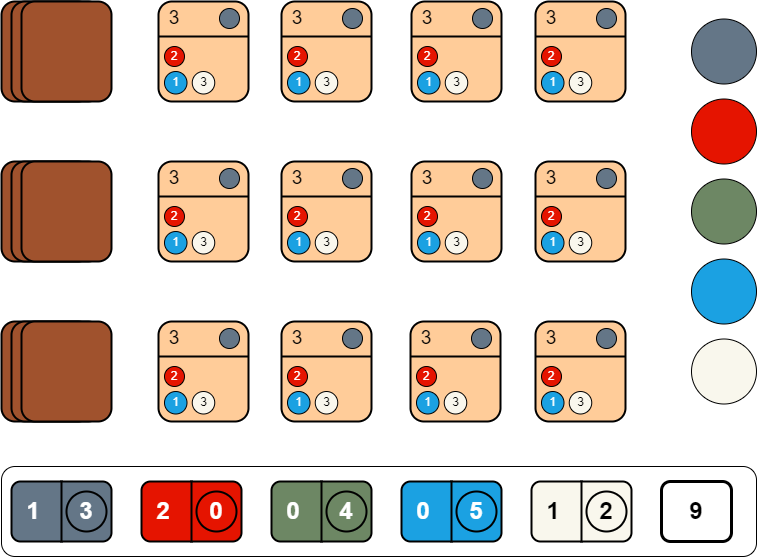
\includegraphics[scale=0.37]{images/screen_structure_plan.png}
\caption{A játék kezdetleges kinézeti terve.}
\label{fig:screen_structure_plan}
\end{figure}


\SubSection{Megvalósítás}

Az idő előrehaladtával formáltam mind a felépítést, mind a kinézetet, de a koncepció alapja megmaradt. A játék kapott egy hozzá illő hátteret, a kártyalapok színét is élőbbé tettem, a zsetonokat a halomban lévő számuk alapján megszámoztam és a zsetongyűjtő panelt is újraterveztem. Létrehoztam egy második panelt is a képernyő felső részén annak érdekében, hogy az adott játékos tudja követni az ellenfél részeredményeit is.
Emellett a jobb felső sarokba elhelyeztem egy "új játék" és egy "Játékszabályok" feliratú gombot, a hozzájuk tartozó funkciók ellátásához. Végezetül pedig megjelöltem a soron lévő játékost a hozzá tartozó panelének körberajzolásával és a játékost jellemző ikonnal.

\begin{figure}[h]
\centering
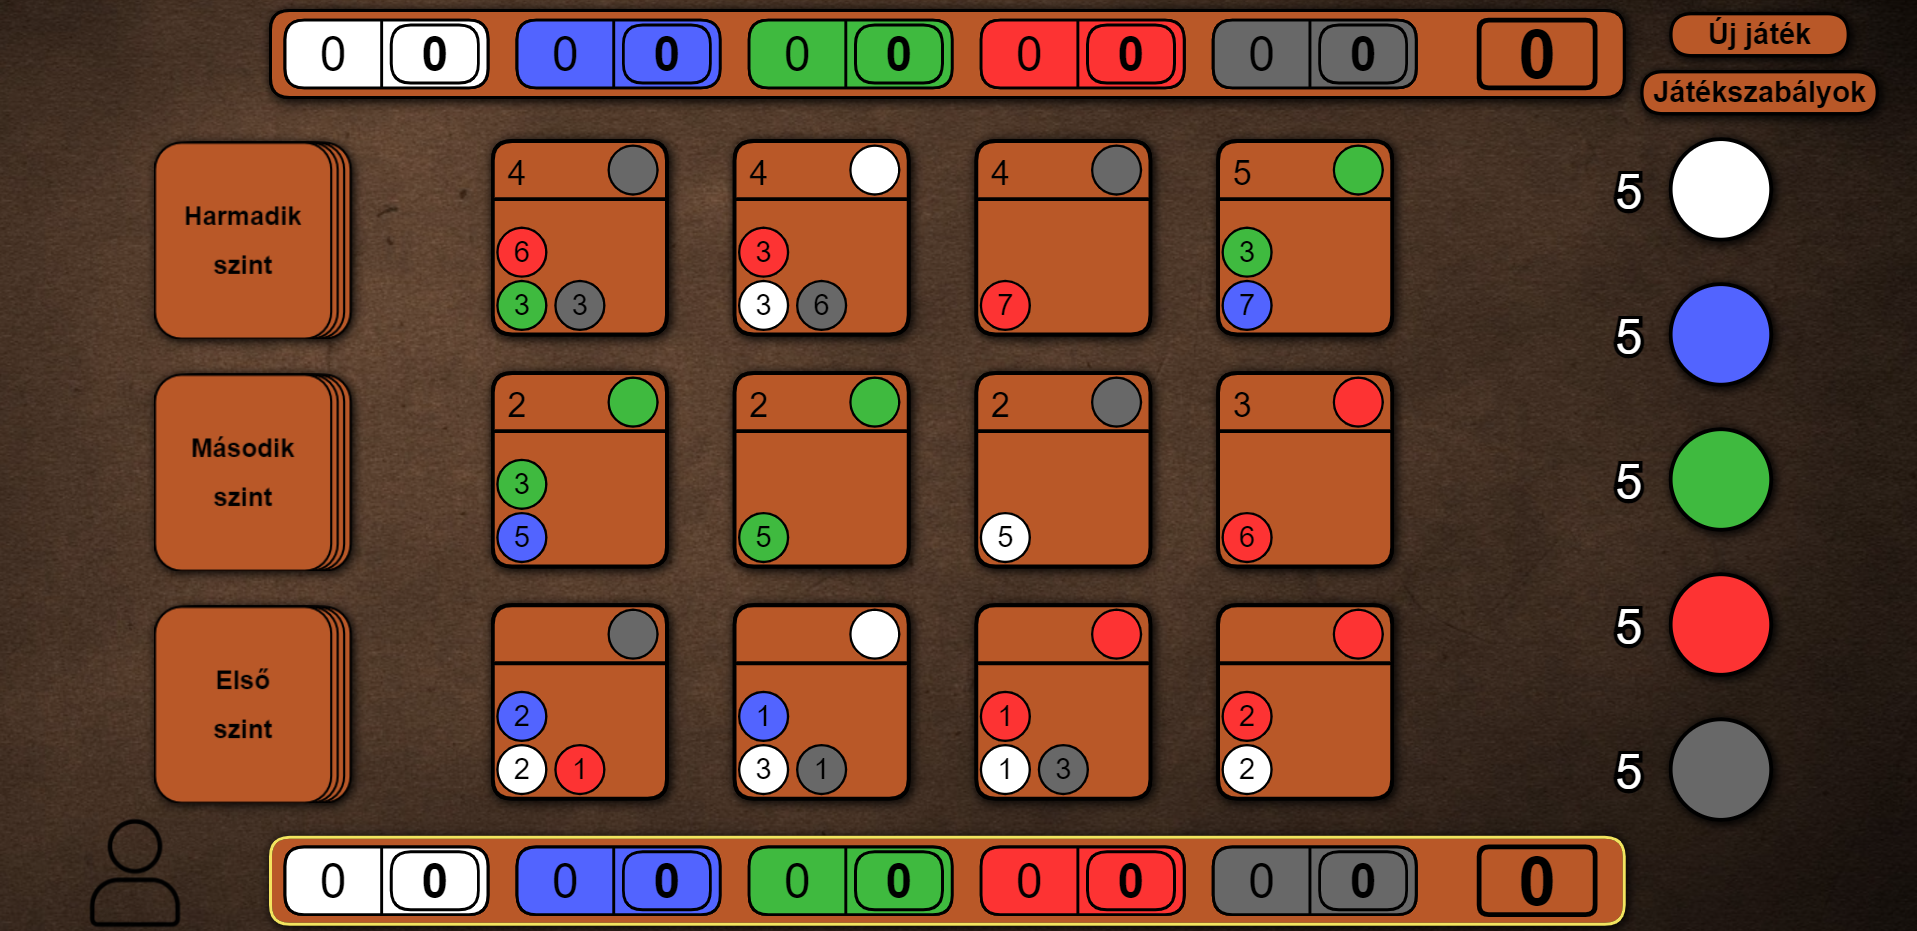
\includegraphics[scale=0.3]{images/screen_structure.png}
\caption{A játék végleges kinézete.}
\label{fig:screen_structure}
\end{figure}


\Section{Alapok}

Az általam leszűkített szabályrendszer alapú játék megvalósításához a JavaScriptet, a megjelenítéséhez pedig főleg a HTML5 Canvast, minimálisan pedig a CSS-t használtam.

\Section{Fáljrendszer kialakítása}

A játék fájlrendszerének alapját egy index nevű html fájl adja, amelyben magát a webes felület hoztam létre. Ide importáltam az összes szükséges JavaScript fájlt és beállítottam, hogy induláskor hívja meg a main.js fájlban meghatározott inicializáló függvényt. A main fájl gyűjti össze az összes funkciót, amit a játék magában foglal. Itt vannak definiálva a canvas alapfüggvényei, például a kattintás, egér mozgatás funkciók, valamint az imént említett inicializáló függvény, ami a canvast és a hozzá tartozó függvényeket érinti. A fájlok mellett van egy data nevű mappa, ahova a játék egész kártyakészletének adatait mentettem. Emellett egy classes nevű mappa is, ahol az objektumok és funkciók szerint szeparált JavaScript osztályok találhatóak. Végezetül pedig egy AI elnevezésű mappa, amelyekbe az általam fejlesztett számítógépes logikák fájljait helyeztem.


\Section{Kártyalapok}

A lapok körvonalát másodfokú görbék segítségével hoztam létre, az ezeken lévő zsetonokat pedig a megfelelő színnel kitöltött körrel valósítottam meg. A pontszámot és a bónusz zsetont jelölő kört egy vonallal választottam el a többi adattól. A pontszám a jobb, a bónusz pedig a bal felső sarkába került a kártyalapnak. A kártya alsó felén helyeztem el a megvásárláshoz szükséges zsetonokat az értékeikkel együtt, úgy, hogy a paraméterként megkapott értékektől függően balról jobbra, lentről felfelé töltődnek fel a pozícióik. Meghatároztam a játék során végig használt alapszínek RGB kódját is.

\Section{Zsetonok}

A zsetonokat körök kirajzolásának segítségével hoztam létre, amelyeket a megfelelő színnel töltöttem ki, és melléjük kiírattam az adott halomban lévő zsetonok számát.


\Section{Zsetongyűjtő panel}

Létrehoztam a panel elemek számára egy osztályt, ahol az adott elem kirajzolását valósítottam meg. A háttérszínét a hozzá tartozó színnel töltöttem ki, két részre osztottam egy függőleges vonallal és a bónusz értéket egy külön körvonallal jelöltem meg. Ezután létrehoztam a panelnek is egy külön osztályt, ahol inicializáltam a különböző panel elemeket, a panel jobb szélén pedig létrehoztam a pont számítására levő elemet. A panel és a panel elemek körvonalát szintén másodfokú görbék segítségével rajzoltam meg.

\Section{Tábla osztály}

A tábla osztályban terveztem összefogni a játék elemeit, és a játék kirajzolásának, működésének, szabályainak megvalósítását. Kezdetben a játék elemeinek elhelyezkedését szerettem volna meghatározni. Kitaláltam a kártyák megfelelő pozícióját és elhelyeztem őket sorban, egyelőre még csak véletlenszerűen az összes kártya közül kiválasztva, nem a megfelelő szintekre bontva. Ezután a panelek, a zsetonok és a kártyapaklik elhelyezése következett, még a megfelelő értékeik nélkül. Majd pedig beállítottam a táblának a hátterét is.

A következő szakaszban a már elhelyezett elemeknek az értékeire helyeztem a hangsúlyt. Igyekeztem a hozzájuk tartozó megfelelő értékeket társítani. Megvalósítottam, hogy a kártyák a szintjeik alapján legyenek kiválogatva külön tömbbe. Ezeket a tömböket megkevertem, majd ebből kihúztam és elhelyeztem a lapokat a játéktérre a játékszabály által leírt módon. A zsetongyűjtő panelre is a hozzá tartozó megfelelő értékeket írtam ki, és a zsetonoknak is megadtam a kezdő értéküket.

\Section{Egér mozgatás}

Ezután a kártyák és a zsetonok egér mozgatásra való interakcióját kezdtem el megvalósítani. Kezdetben egérkattintásra néztem meg, hogy a kártyákra és zsetonokra kattintva a megfelelő indexű és koordinátájú elemet kapom-e vissza. Azt, hogy az egér beleesik-e az adott kártya vagy zseton területébe a koordinátájukból, a magasságukból és a szélességükből kiszámítva határoztam meg. Kezdetben a tábla osztályban egy függvényben határoztam ezt meg, később viszont a kártya saját osztályában, önmaga dönti el, hogy éppen a kurzor alatt van-e vagy sem. Ezután a már működő programrészt átültettem az egér mozgatására és megjelöltem az egér alatt lévő elemet úgy, hogy a körvonalát egy világos, sárga színnel rajzoltam körbe. Emellett a kurzor típusát is átállítottam az esetben, amikor egy kártya vagy zseton felett van.

\Section{Interakciók}

A játékon belüli interakciókat a zsetonvásárlással és az ennek hatására történő panel értékek feltöltésével kezdtem. Ezt úgy valósítottam meg, hogy a korábban meghatározott egér kattintáskor kiszámolt zseton értéket megkapva, a megfelelő színű halmot csökkentettem, a panelen viszont növeltem ezt az értéket.

Ezután a kártyavásárlással járó történésekkel foglalkoztam. Kezdetben azt valósítottam meg, hogy kattintáskor a kurzor alatt található kártya eltűnjön, majd a helyére a megfelelő, megkevert részpakliból kerüljön a következő lap. A bónusz értékek megszerzését is feltüntettem a panelen. A birtokba vétel után, a kártyán található pontszám (amennyiben van) hozzáadódik a panelen található játékos pontszámához. A zsetonok a szabályok alapján olyan módon kerülnek vissza a halmokba, hogy ami felhasználásra került, azt mind vissza kell szolgáltatni a játéktérre, ami viszont bónusz, az a játékos birtokában marad. Amennyiben több zsetonnal rendelkezett a játékos az adott színből, mint amennyire a kártya megvásárlásakor szükség volt, a bónuszok közül az összes és a zsetonok közül a szükséges mennyiség kerül felhasználásra, így a többlet érték a játékosnál marad zseton formájában.


\Section{Szabályrendszer}

A szabályrendszer megalkotásának szempontjából a kártyák és a zsetonok elérhetősége jelenti az alapot, így ezek  lefektetésével kezdtem neki ennek a területnek.

A szabályok alapján akkor lehet megvásárolni egy kártyát, ha a játékos birtokában van a lapon feltüntetett zsetonszám a megadott színekből, akár zsetonokból, akár a korábban megszerzett bónuszokból kifizetve azt. Valamint fontos, hogy kártyavásárlás esetén mást nem csinálhat a körében és amennyiben felvett egy zsetont, visszafordítani nem tudja az eseményeket.

A zsetonok kiválasztása ennél egy fokkal bonyolultabb. Alapvetően egy zseton akkor elérhető a játékos számára, ha az adott halomban legalább egy található, ezen felül viszont a zsetonhúzás két féle módon tud történni egy kör során. Az első esetben a játékos három zsetont választ, amelyek közül mindegyik különböző színű, a második lehetőség pedig, hogy két azonos színű zsetont választ, de ezt csak abban az esetben tudja megtenni, ha az adott halomban a kör elején legalább négy zseton található.

Ezeknek a feltételrendszereknek a megvalósítása külön függvényekben történik, amelyeket a kártyára vagy a zsetonra való kattintáskor ellenőriz a program, hogy elérhető-e az adott játékos számára. Fontos, hogy az egy körön belül lévő korábbi cselekvéseink is korlátozhatják a lehetőségeinket, tehát ha zsetont vesz fel a játékos az első cselekvésekor, a kártyaválasztás már nem elérhető a számára. A zsetonok között is fellelhető ez a jelenség, például amikor kiválasztunk két különböző színű zsetont, azok már biztosan nem elérhetőek az adott körben, akármennyi is van a halomban, hiszen csak a három eltérő színű zsetonválasztás típusú lépéssorozat folytatható. Ezen felül a korábbi körök lépései is befolyásolják és akár korlátozzák a lehetőségeinket. Amikor a kör kezdetén egy három zsetont tartalmazó halomból húzunk fel egyet, az már továbbra nem elérhető számunkra a kör során, mivel kettő felhúzása nem lehetséges a zsetonszám miatt. Továbbá a kifogyott halmok sem elérhetőek a játékosok számára, így akár felmerülhet olyan esemény, amikor a három különböző színű zseton felvételekor nem elérhető a maximális számú lehetőség, így csak annyit vehetünk fel, amennyi a rendelkezésünkre áll a szabályok szerint.

\Section{Körökre osztás}

A játékot az aktuális játékos indexe alapján bontottam körökre. Létrehoztam a játékos osztályt a megfelelő értékekkel és inicializáltam őket a tábla osztályon belül a többihez hasonlóan, összekapcsolva a hozzájuk tartozó panelekkel. Bevezettem a kattintások dokumentálására egy változót, amelyben eltároltam az éppen játékban lévő játékos a köre megkezdésétől megtett, a szabályok és a játék akkori állása alapján megengedett kattintásait. A kártya vásárlásakor az indexe, a zseton megvásárlásakor pedig a színe kerül bele. Ezen információk segítségével ítéli meg a program, hogy vége van-e az adott játékos körének. Amikor az első cselekvés kártyavásárlás volt, a kör azonnal átadódik a másik játékosnak. Ellenkező esetben figyeli a kattintások tömbjét. Amennyiben kettő azonos színű zseton lett kiválasztva, szintén a következő játékosra vált. Az utolsó lehetőség esetén pedig ellenőrzi, ha az első és a második választott zseton színe nem egyezik, akkor a harmadiknak sem szabad egyeznie egyikkel sem, miután pedig ez megfelelt a kritériumoknak a kör szintén a következő játékosé lesz.

\Section{Ablakátméretezés}

Az ablakátméretezés problémáját is meg szerettem volna oldani, hogy akármilyen ablakméretnél lehessen játszani a játékkal. Ezt az ablak koordinátáinak ellensúlyozásával, transzformálásával és skálázásával oldottam meg. Az alábbi képeken látható, hogy miként néz ki a játéktér különböző ablakméretek mellett.

\begin{figure}[h]
\centering
$\vcenter{\hbox{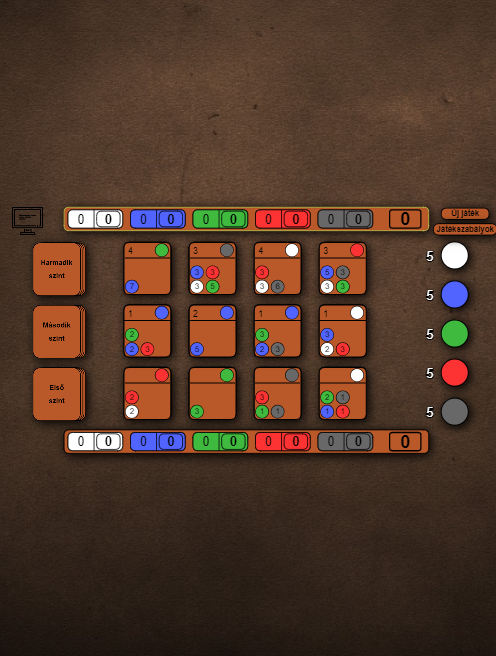
\includegraphics[scale=0.2]{images/resize1.png}}}$
\hspace{1cm}
$\vcenter{\hbox{
\includegraphics[scale=0.2]{images/resize2.png}}}$
\caption{A játék kinézete különböző ablakméret mellett.}
\label{fig:resize}
\end{figure}

\Section{Esztétikai beállítások}

A játéktéren található elemek formázását a Canvas segítségével, az ezen kívül található (például a kezdőképernyő, játék végén felugró felület, stb.) felületek formázását viszont CSS segítségével valósítottam meg. Azért követtem ezt a logikát, hiszen a játéktéren, a játékmenettel kapcsolatos dolgok összetartoznak és jó, ha egy logika alapján vannak formázva, míg az ezen kívüli elemek egy másik csoportot alkotnak, amelyeket egyszerűbbnek tartottam CSS-ben megvalósítani.

\SubSection{Játékos számára releváns információk}

Kiemeltem grafikusan a játékosok számára fontos információkat, ezáltal jobban átláthatóbbak a lehetőségek. Zöld színű, vékony vonallal körberajzoltam az elérhető kártyákat, az éppen nem elérhető zsetonoknak viszont szürke körvonalat adtam, így az egér mozgatására sem látható a kiválaszthatóságuk. Az éppen körön lévő játékos paneljét is egy vékony, sárga vonallal rajzoltam körbe, valamint a képernyő bal oldalán, az aktuális panel mellet megjelenítettem egy játékost jellemző ikont is, így egyértelműbbé válik, hogy melyik játékos van soron.

\SubSection{Kezdőképernyő}

Ezután megalkottam és megformáztam a kezdőképernyőt, ami minden játékindításkor megjelenik a felhasználó számára. Ennek a felületnek az alapja a játék táblájának elhomályosítása, amelyen egy kiírás és két gomb található. A felirat felszólítja a játékost, hogy válassza ki az adott játékban szereplő játékosokat. A két gomb a két lehetőséget reprezentálja, miszerint vagy két emberi, vagy pedig egy emberi és egy számítógép által vezérelt játékos fog játszani. Ezeknek a megjelenítését és az eseménykezelését CSS segítségével valósítottam meg.


\SubSection{Gomb interakciók}

Ez követően a játéktéren található gombokkal foglalatoskodtam, amelyeknek létrehoztam egy külön osztályt a megfelelő paramétereikkel, tehát ezeket a gombokat az előzőkkel ellentétben a Canvas segítségével valósítottam meg. Először csináltam egy "Új játék" feliratú gombot, amellyel a játék során akármikor új játékot lehet kezdeni. Ezt követően pedig a hasonló felépítésű "Játékszabályok" elnevezésű gombot helyeztem el a képernyőn, amelyre való kattintással egy olyan felület jön elő, ahol a játékszabályokat olvashatjuk el. Ez a felugró felület CSS-ben lett megalkotva. Az alap szintén az elhomályosított tábla, amelyen egy kerettel és háttérrel rendelkező felirat doboz helyezkedik el. Ezen a felületen található az általam megvalósított játékverzió szabályai. Ebből a felületből való kilépést az elhomályosított területre való kattintással valósítottam meg. A tábla elemekhez hasonlóan a kurzor mozgatásra reagáló megjelenést hoztam létre a gombok számára is, miszerint a betűszínük sárgával van átrajzolva, amennyiben az egér alatt találhatók.


\SubSection{Elérhető lépések megszűnése}

Ahogy korábban is említettem, a játékszabályok módosításával sajnos felmerülhet egy olyan játékállapot, amikor az adott játékos sem kártyát, sem zsetont nem tud választani. Ezt az eshetőséget a korábbiakhoz hasonlóan olyan formában orvosoltam, hogy a jelenség bekövetkezésekor megjelenik egy szöveg, amely tájékoztatja a játékost a felmerült problémáról, és arról, hogy ennek az üzenetnek a bezárása után újraindul a játék.

\newpage

\SubSection{Záró képernyő}

A játék végét jelentő feltételt követően pedig megjelenik a záró képernyő, amelyen látható egy felirat és egy gomb. A szöveg tájékoztatja a felhasználót arról, hogy melyik játékos nyerte a játékot, a gomb pedig lehetőséget ad a játék újrakezdésére, amely megnyomásával megjelenik a kezdőképernyő. Ezt a felületet a kezdőképernyőhöz hasonlóan formáztam meg mind a hátteret, mind a feliratot, mind a gombot tekintve.

\SubSection{Esztétika és refaktorálás}

A játék fejlesztésének egészében folyamatosan zajlottak a kódrészek átszervezései, refaktorálása, egyszerűbbé, egyértelműbbé tétele, valamint az esztétikai fejlesztések, javítgatások. Ahogy viszont többek között a tábla osztályon is észrevehető, ezek a folyamatok azonban nincsenek maradéktalanul elvégezve, ami a program szempontjából a megvalósított játékszabályok és funkciók bővítése mellett továbbfejlesztési lehetőségek.

\Section{Osztálydiagram}

\begin{figure}[h]
\centering
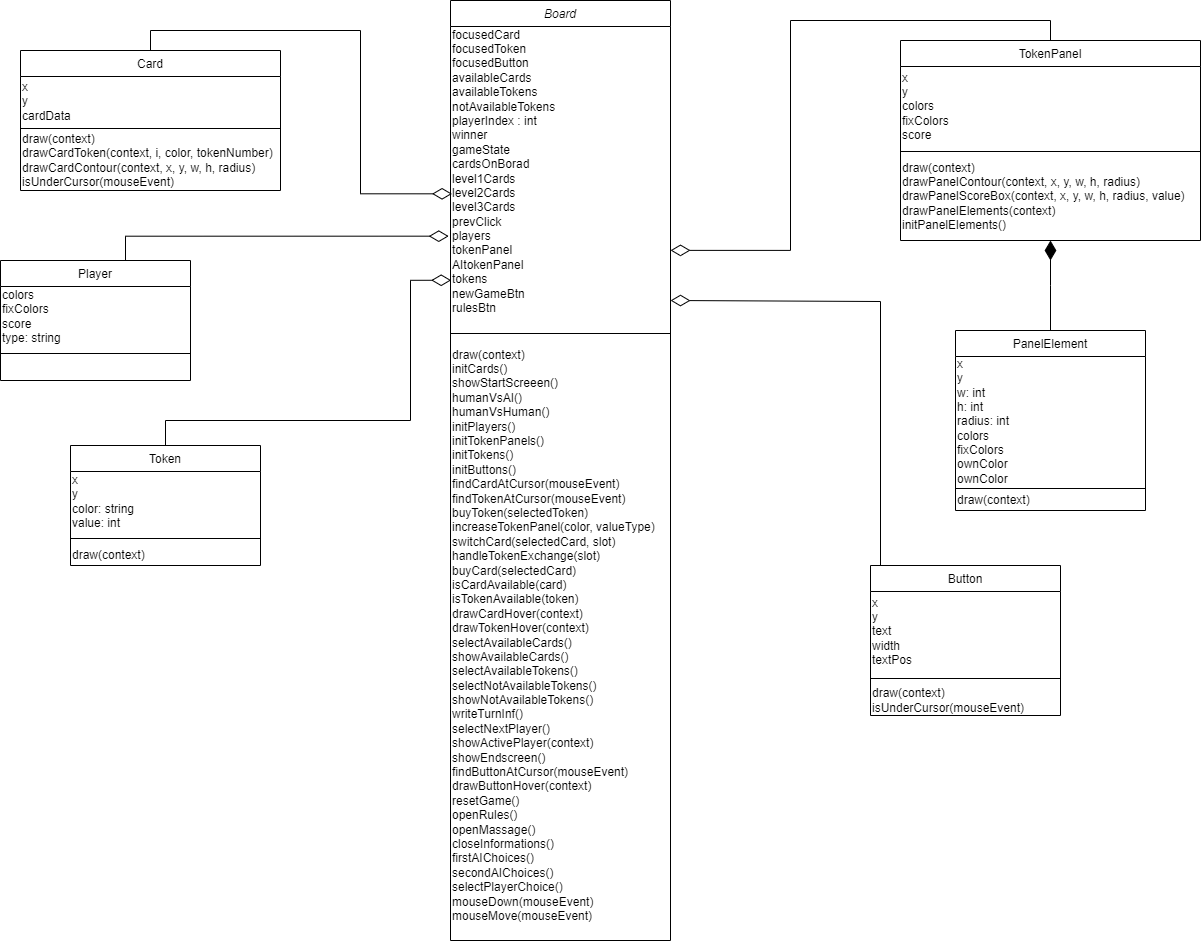
\includegraphics[scale=0.35]{images/UML.png}
\caption{A játék megvalósításának osztálydiagramja.}
\label{fig:uml}
\end{figure}


\include{chapters/5_Ai}
\Chapter{Szimulációk}

A megvalósított mesterséges intelligenciák erősségének összeméréséhez szimulációkra volt szükség. A fejezetben ezen vizsgálatok elvégzésének módját, a kapott eredményeket és értékelésüket láthatjuk.

\Section{Szimuláció program}

A szimulációk elvégzéséhez egy külön programot hoztam létre, amelyben a különböző AI-okat játszattam egymás ellen. Ezeknek a szimulációknak az eredményét kezdetben a konzolra írtam ki, hogy fel tudjam mérni a különböző AI-ok képességeit.

\SubSection{AI1 az AI2 ellen}

A szimulációk elvégeztével egyértelműen látszott, hogy a második sokkal eredményesebb mint az első, hiszen általánosan körülbelül a 85\%-át tudta megnyerni a lejátszott játékoknak.

Különböző vizsgálatokat futtattam a két AI játszmáinak kapcsán. Először azt vizsgáltam, hogy milyen a lejátszott meccsek végén a játékosok összpontszámának gyakoriság hisztogramja tízezer játék esetén (\ref{fig:scores1v2}. ábra). Az ábrán látható, hogy az eloszlása közel normálisnak tekinthető, a várható értéke 25.29, a minimuma 15, a maximuma pedig 33.

\begin{figure}[H]
\centering
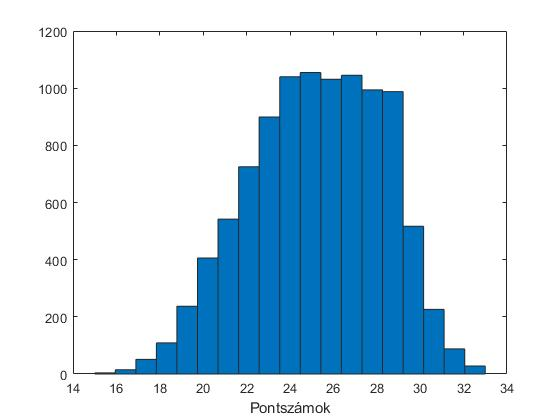
\includegraphics[scale=0.6]{images/final_scores_AI1vsAI2.jpg}
\caption{Az első és második AI összpontszámainak eloszlása.}
\label{fig:scores1v2}
\end{figure}


Egy hasonló vizsgálat során, ugyanezen játékszám mellett a lejátszott meccsek köreinek számát tekintve vizsgáltam meg a gyakoriság hisztogramját (\ref{fig:rounds1v2}. ábra). Ezen ábrán is látható, hogy a körök száma is normálisnak tekinthető, várható értéke 63.86, minimuma 43 és a maximuma 89. Érdekes módon hatvanhét és hatvannyolc közé nem esett egy darab körszám sem.

\begin{figure}[H]
\centering
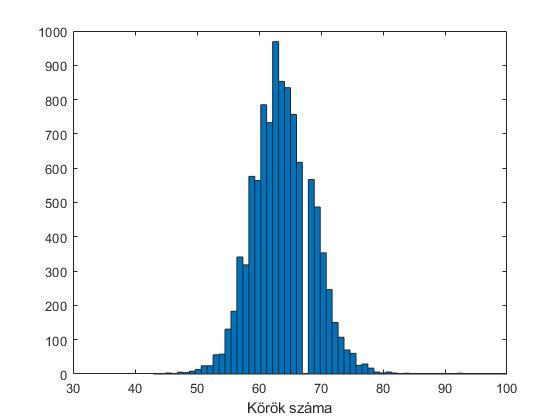
\includegraphics[scale=0.6]{images/round_number_hist_AI1vsAI2.jpg}
\caption{Az első és második AI köreinek eloszlása.}
\label{fig:rounds1v2}
\end{figure}

Végezetül pedig egy játékban a pontszámaiknak növekedését elemeztem. (\ref{fig:player_scores1v2}. ábra). Az ábrán jól látható, hogy mivel az első AI teljesen véletlenszerűen választ kártyákat, így a játék késői fázisában is csak alacsony szintű lapokat vásárol, pedig lehet, hogy elérhetőek lennének számára magasabb szintűek is. Ezen okból a második algoritmus főként a játék második felében kiemelkedően az első felé tud kerekedni.

\begin{figure}[H]
\centering
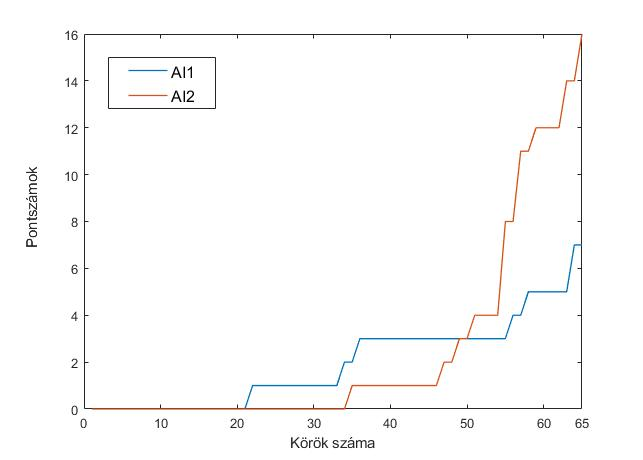
\includegraphics[scale=0.6]{images/player_points_AI1vsAI2.jpg}
\caption{Az első és második AI pontszámainak növekedése.}
\label{fig:player_scores1v2}
\end{figure}

\SubSection{AI2 az AI3 ellen}

A szimulációk elvégzése után láthatóvá vált, hogy a második algoritmus nagyobb arányban tudott nyerni, mint a harmadik. Körülbelül 74\%-ban nyert a második a harmadikkal szemben. Ebből az a következtetés vonható le, hogy a lapválasztást tekintve érdemesebb mindig a lehető legmagasabb szintű lapot választani a játék megnyerése érdekében. Az eredmények tekintetében a harmadik helyett továbbra is a második AI logikáját vettem alapul a következő algoritmus megvalósításakor a kártyaválasztásra nézve.

\SubSection{AI2 az AI4 ellen}

Ahogy elvégeztem a szimulációkat, kiderült, hogy a második logika ez esetben is nagyobb arányban tudott nyerni, mint a negyedik. Általánosan 57\%-kát tudta megnyerni a lejátszott meccseknek. Az, hogy a negyedik algoritmus nem hatékony abból fakad, hogy a játék előrehaladtával a késői fázisban is csak azt nézi, hogy melyik a számára legkönnyebben elérhető lap, így az alacsony szintűekre kezd el gyűjteni, nem pedig az értékesebb lapokra, így a pontszerzés szempontja a háttérbe szorul. Ezért tud az AI2 az AI4 fölé kerekedni.

A konklúzió, hogy a második algoritmus eredményesebb volt a harmadiknál és a negyediknél egyaránt. Ezáltal sem a kártyaválasztás, sem a zsetonválasztás terén nem sikerült előrelépni.

\SubSection{AI2 az AI5 ellen}

Az ötödik AI megvalósítása során figyelembe véve az előző próbálkozások (AI3, AI4) kvázi sikertelenségeit, igyekeztem azokból tanulva kiküszöbölni azok buktatóit, ezáltal a kártya-, és zsetonválasztás terén egyaránt előrelépést elérni a másodikhoz képest.

Az AI elkészítése után lefuttatva a szimulációkat kiderült, hogy a fejlesztéseim sikeresek voltak.
Az ötödik algoritmus körülbelül annyival erősebb, mint amennyivel a második volt az elsőtől. Általánosan 86\%-kát nyeri meg a lejátszott játékaiknak. Ez bizonyult tehát a legeredményesebb logikának a szimulációim során.

Az elsőhöz hasonlóan megnéztem, hogy miként alakul a játékok végén a játékosok összpontszámainak gyakoriság hisztogramja szintén tízezer játszma esetén (\ref{fig:scores2v5}. ábra). Az előzőhöz hasonlóan az eloszlás közel normálisnak tekinthető, a várható értéke 24.9, a minimuma 15, a maximuma pedig 33.

\begin{figure}[H]
\centering
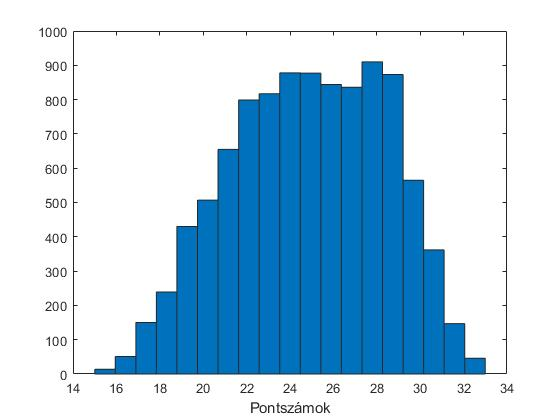
\includegraphics[scale=0.6]{images/final_scores_AI2vsAI5.jpg}
\caption{A második és ötödik AI összpontszámainak eloszlása.}
\label{fig:scores2v5}
\end{figure}

A következő vizsgálat során tízezer játékszám mellett a lejátszott meccsek köreinek számát tekintve vizsgáltam meg a gyakoriság hisztogramját, ahogy korábban is tettem (\ref{fig:rounds2v5}. ábra). Az eloszlás ez esetben lényegesen különbözik, ennek oka: a két mesterséges intelligencia erőssége jelentősen eltér.

\begin{figure}[H]
\centering
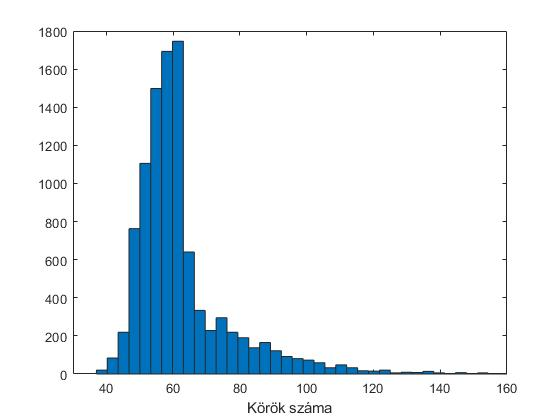
\includegraphics[scale=0.6]{images/round_number_hist_AI2vsAI5.jpg}
\caption{A második és ötödik AI köreinek eloszlása.}
\label{fig:rounds2v5}
\end{figure}

Ezután pedig az egy játékban való pontjaiknak a növekedését is szintén megvizsgáltam (\ref{fig:player_scores2v5}. ábra). Ezen az ábrán látható, hogy a második AI korábban tud elkezdeni pontot érő lapokat vásárolni, viszont észrevehető, hogy az ötödik egyből egy nagyobb értékűt vásárolt meg, amelyre a korábbi körökben gyűjtött zsetonokat és bónuszokat. Ezt követően pedig újra gyűjteni kezdett a következőre. Ezen logika mentén magasan felül tud kerekedni a második AI-on és az előző ilyen vizsgálathoz képest majdnem tíz körrel hamarabb be is tudta fejezni a játékot.

\begin{figure}[H]
\centering
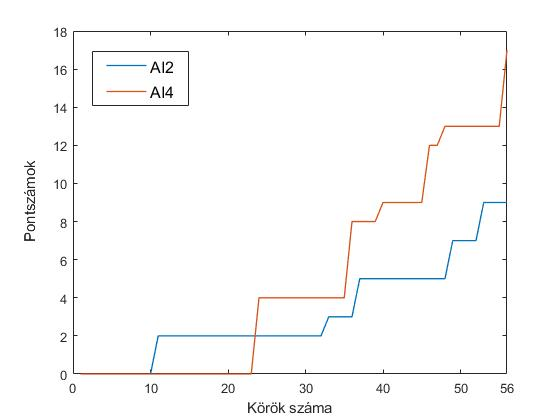
\includegraphics[scale=0.6]{images/player_points_AI2vsAI5.jpg}
\caption{A második és ötödik AI pontszámainak növekedése.}
\label{fig:player_scores2v5}
\end{figure}

\SubSection{Hatékonyság}

Végezetül összegyűjtöttem egy táblázatba a különböző AI-ok hatékonyságát az egymással futtatott szimulációk során. Az eredmények \aref{tab:ai_comparison}. táblázatban láthatók, ennek elkészítéséhez olyan módon módosítottam a kódomat, hogy mindig egy adott algoritmus kezdte a játékokat. A sorok mutatják, hogy melyik AI kezdett, valamint, hogy milyen százalékban tudta megnyerni a játszmákat a többivel összemérve.

\begin{table}[h]
\caption{A gépi intelligenciák eredményessége az egymás elleni szimulációkban.}
\label{tab:ai_comparison}
\medskip
\centering
\begin{tabular}{|c|c|c|c|c|c|} 
 \hline
  & AI1 & AI2 & AI3 & AI4 & AI5 \\ 
 \hline
 AI1 & 55\% & 18\% & 40\% & 22\% & 5.5\%\\ 
 \hline
 AI2 & 86\% & 56\% & 78\% & 62\% & 17\%\\ 
 \hline
 AI3 & 67\% & 30\% & 55\% & 35\% & 8.5\%\\ 
 \hline
 AI4 & 85\% & 50\% & 74\% & 56\% & 12\%\\ 
 \hline
 AI5 & 96\% & 88\% & 95\% & 92\% & 52\%\\
 \hline
\end{tabular}
\end{table}

A tesztek elvégzése után az a következtetés vonható le, hogy a körkezdésnek viszonylag nagy jelentősége van a nyerési arány tekintetében, hiszen ahogy az első algoritmusnál is láthatjuk körülbelül öt százalékkal eredményesebb volt önmagával szemben az, amelyik kezdett. Ez a randomizálás visszaszorulásával arányosan csökken, ha megnézzük az ötödik AI esetét, ahol nagyobb szerepet kap a következetesség. Ebben az esetben már csak két százalékkal volt jobb a körkezdő algoritmus.

A második és a negyedik logika erősségének összemérése esetén ez a jelenség meglepően befolyásolta az eredményt. A korábbi tesztek során kiderült, hogy a második erősebbnek bizonyult, mint a negyedik AI. Ezzel szemben azokban az esetekben, amikor a negyedik kezdett, körülbelül azonos volt a nyerési arányuk.

A táblázat alapján nyerési átlagukból kiszámítva felállítottam egy erősségi sorrendet a különböző AI-ok között. \Aref{tab:ai_ranking}. táblázat fentről lefelé csökkenő sorrendben mutatja a erősorrendet, a jobb oszlopban pedig az látható, hogy az aktuális logika átlagosan milyen arányban tudott nyerni a különböző algoritmusokkal szemben. A \textit{(K)} jelzés azt az esetet jelöli, amikor az adott AI kezdte a játszmákat.

\begin{table}[H]
\caption{A gépi intelligenciák erősorrendje. (A zárójelben a K jelzi, hogy az adott AI kezdi-e a játékot.)}
\label{tab:ai_ranking}
\medskip
\centering
\begin{tabular}{|l|c|} 
\hline
Név & Átlag \\
 \hline
 AI5 (K) & 93\%\\ 
 \hline
 AI5 & 90\%\\ 
 \hline
 AI2 (K) & 61\%\\ 
 \hline
 AI4 (K) & 55\%\\ 
 \hline
 AI2 & 53\%\\
 \hline
  AI4 & 47\%\\ 
 \hline
 AI3 (K) & 35\%\\ 
 \hline
 AI3 & 28\%\\ 
 \hline
 AI1 (K) & 22\%\\ 
 \hline
 AI1 & 16\%\\
 \hline
\end{tabular}
\end{table}
\Chapter{Összefoglalás}

Hasonló szerepe van, mint a bevezetésnek.
Itt már múltidőben lehet beszélni.
A szerző saját meglátása szerint kell összegezni és értékelni a dolgozat fontosabb eredményeit.
Meg lehet benne említeni, hogy mi az ami jobban, mi az ami kevésbé jobban sikerült a tervezettnél.
El lehet benne mondani, hogy milyen további tervek, fejlesztési lehetőségek vannak még a témával kapcsolatban.

\appendix
\chapter{Algoritmusok folyamatábrái}

\begin{figure}[h]
\centering
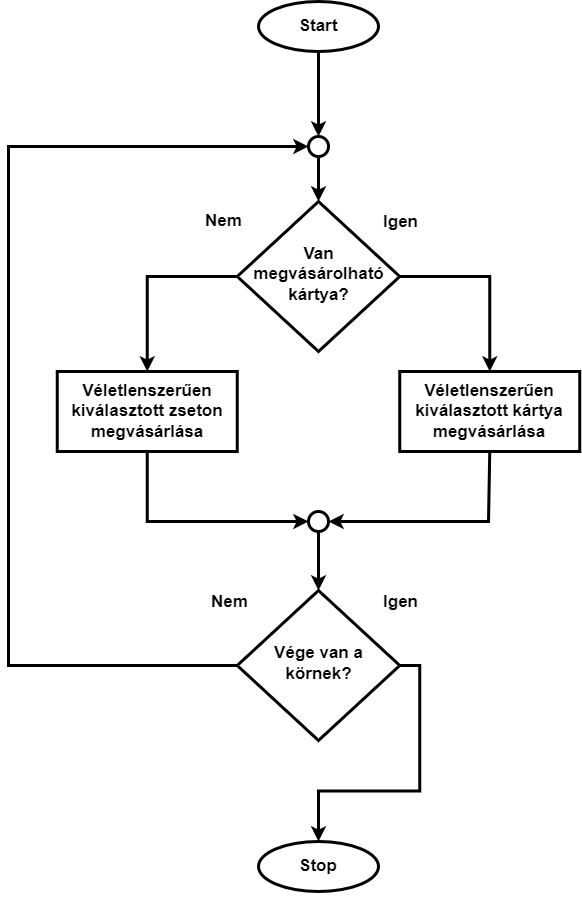
\includegraphics[scale=0.5]{images/firstAI_flowchart.png}
\caption{Az AI1 folyamatábrája.}
\label{fig:AI1_flowchart}
\end{figure}

\begin{figure}[h]
\centering
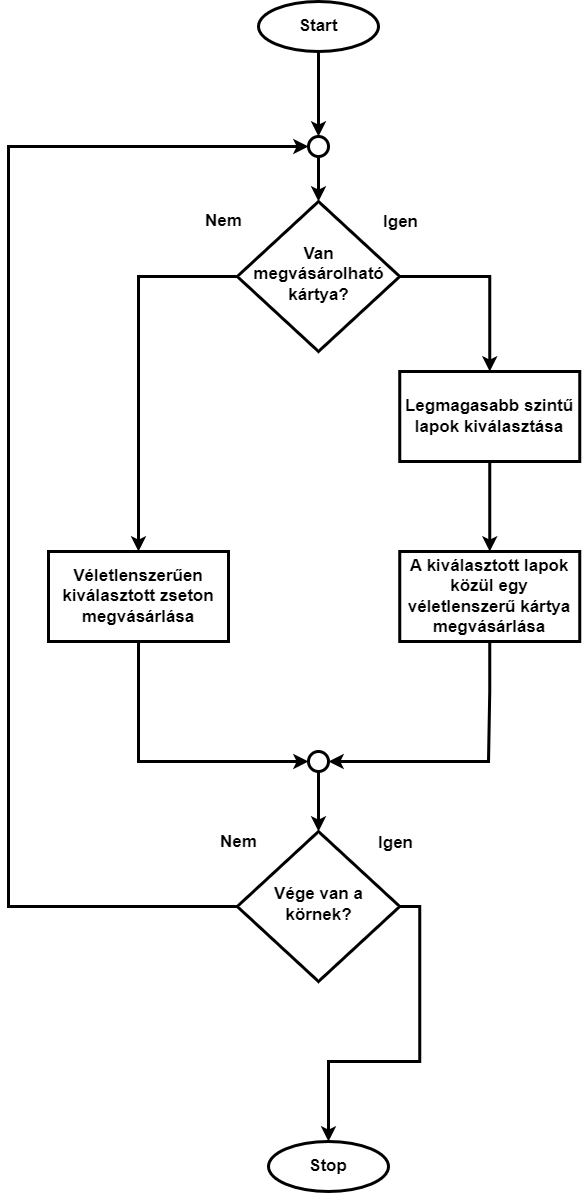
\includegraphics[scale=0.5]{images/secondAI_flowchart.png}
\caption{Az AI2 folyamatábrája.}
\label{fig:AI2_flowchart}
\end{figure}

\begin{figure}[h]
\centering
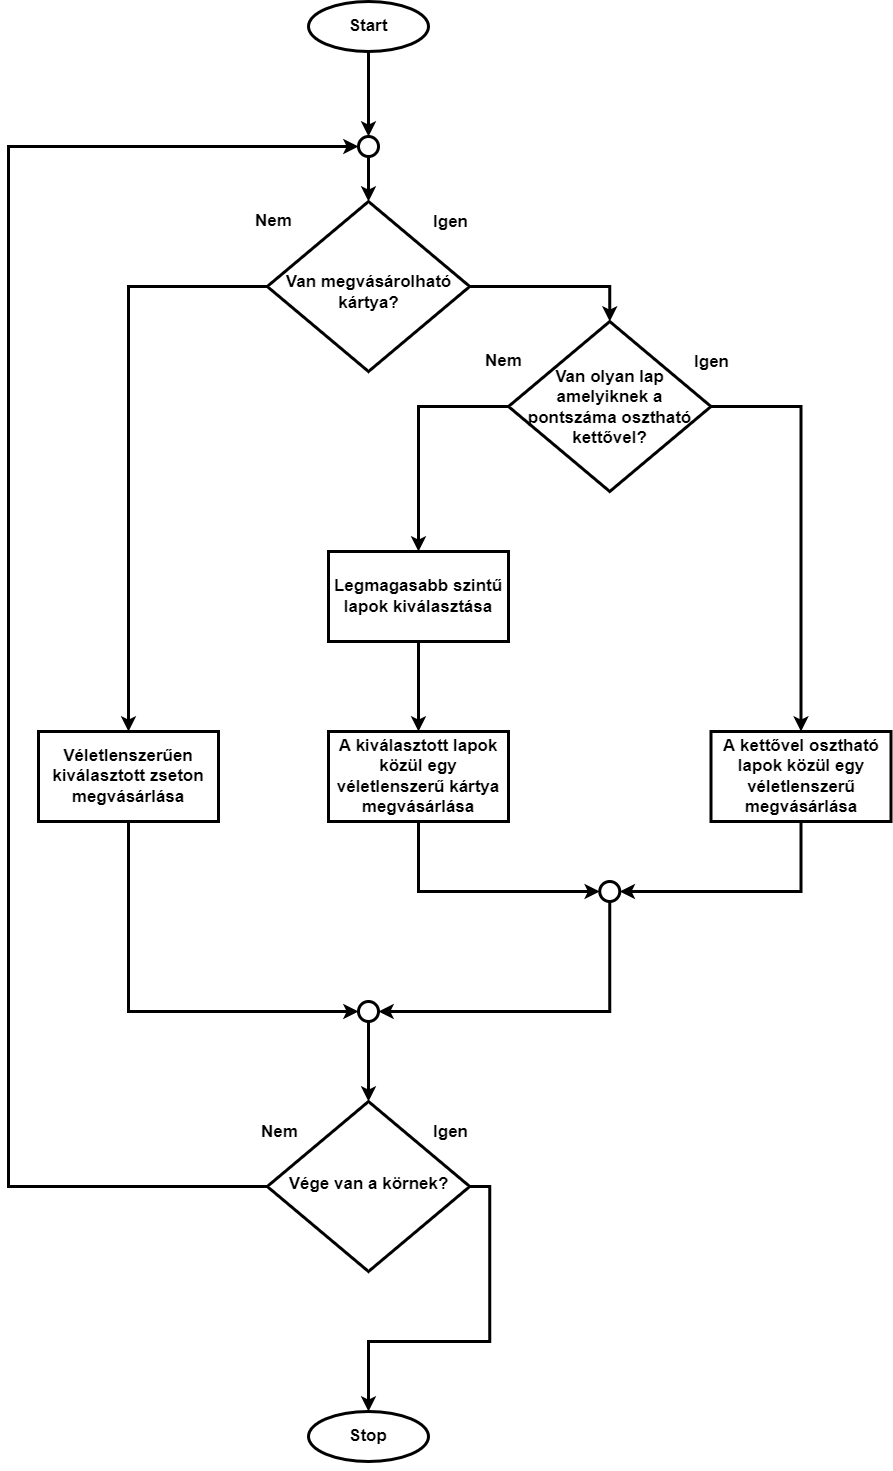
\includegraphics[scale=0.4]{images/thirdAI_flowchart.png}
\caption{Az AI3 folyamatábrája.}
\label{fig:AI3_flowchart}
\end{figure}

\begin{figure}[h]
\centering
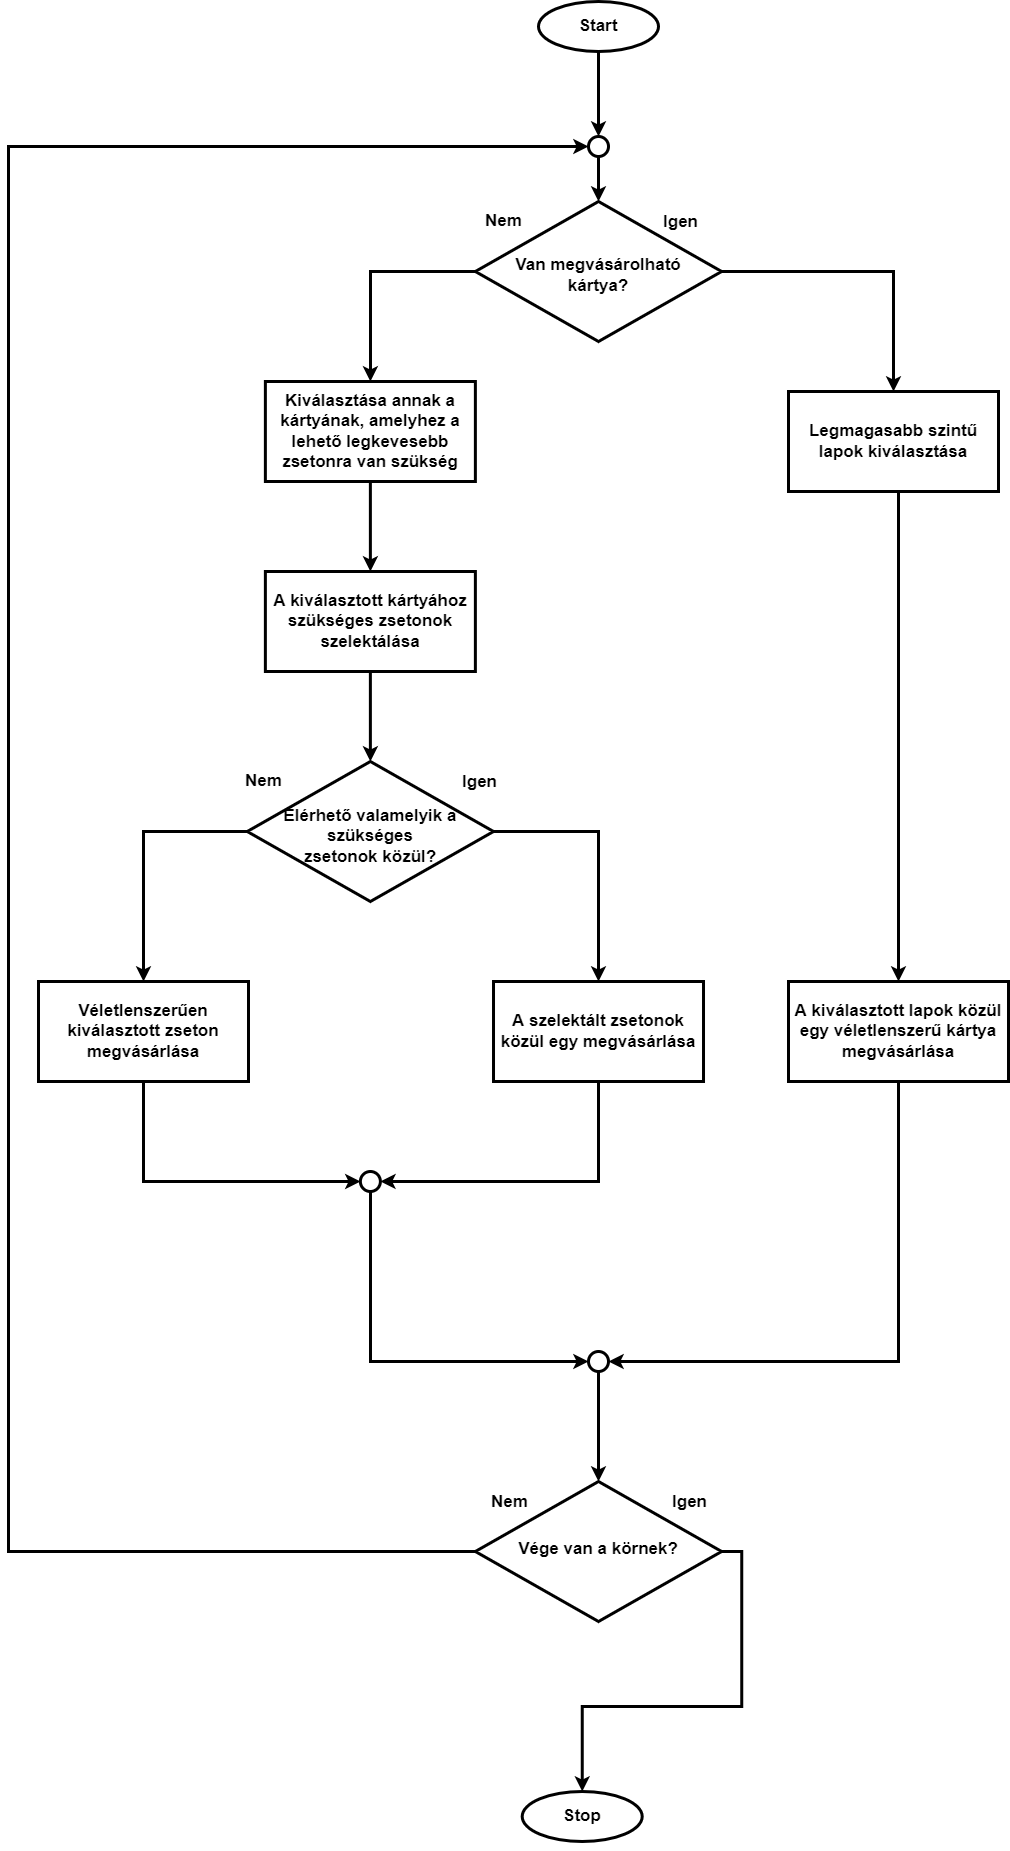
\includegraphics[scale=0.35]{images/fourthAI_flowchart.png}
\caption{Az AI4 folyamatábrája.}
\label{fig:AI4_flowchart}
\end{figure}

\begin{figure}[h]
\centering
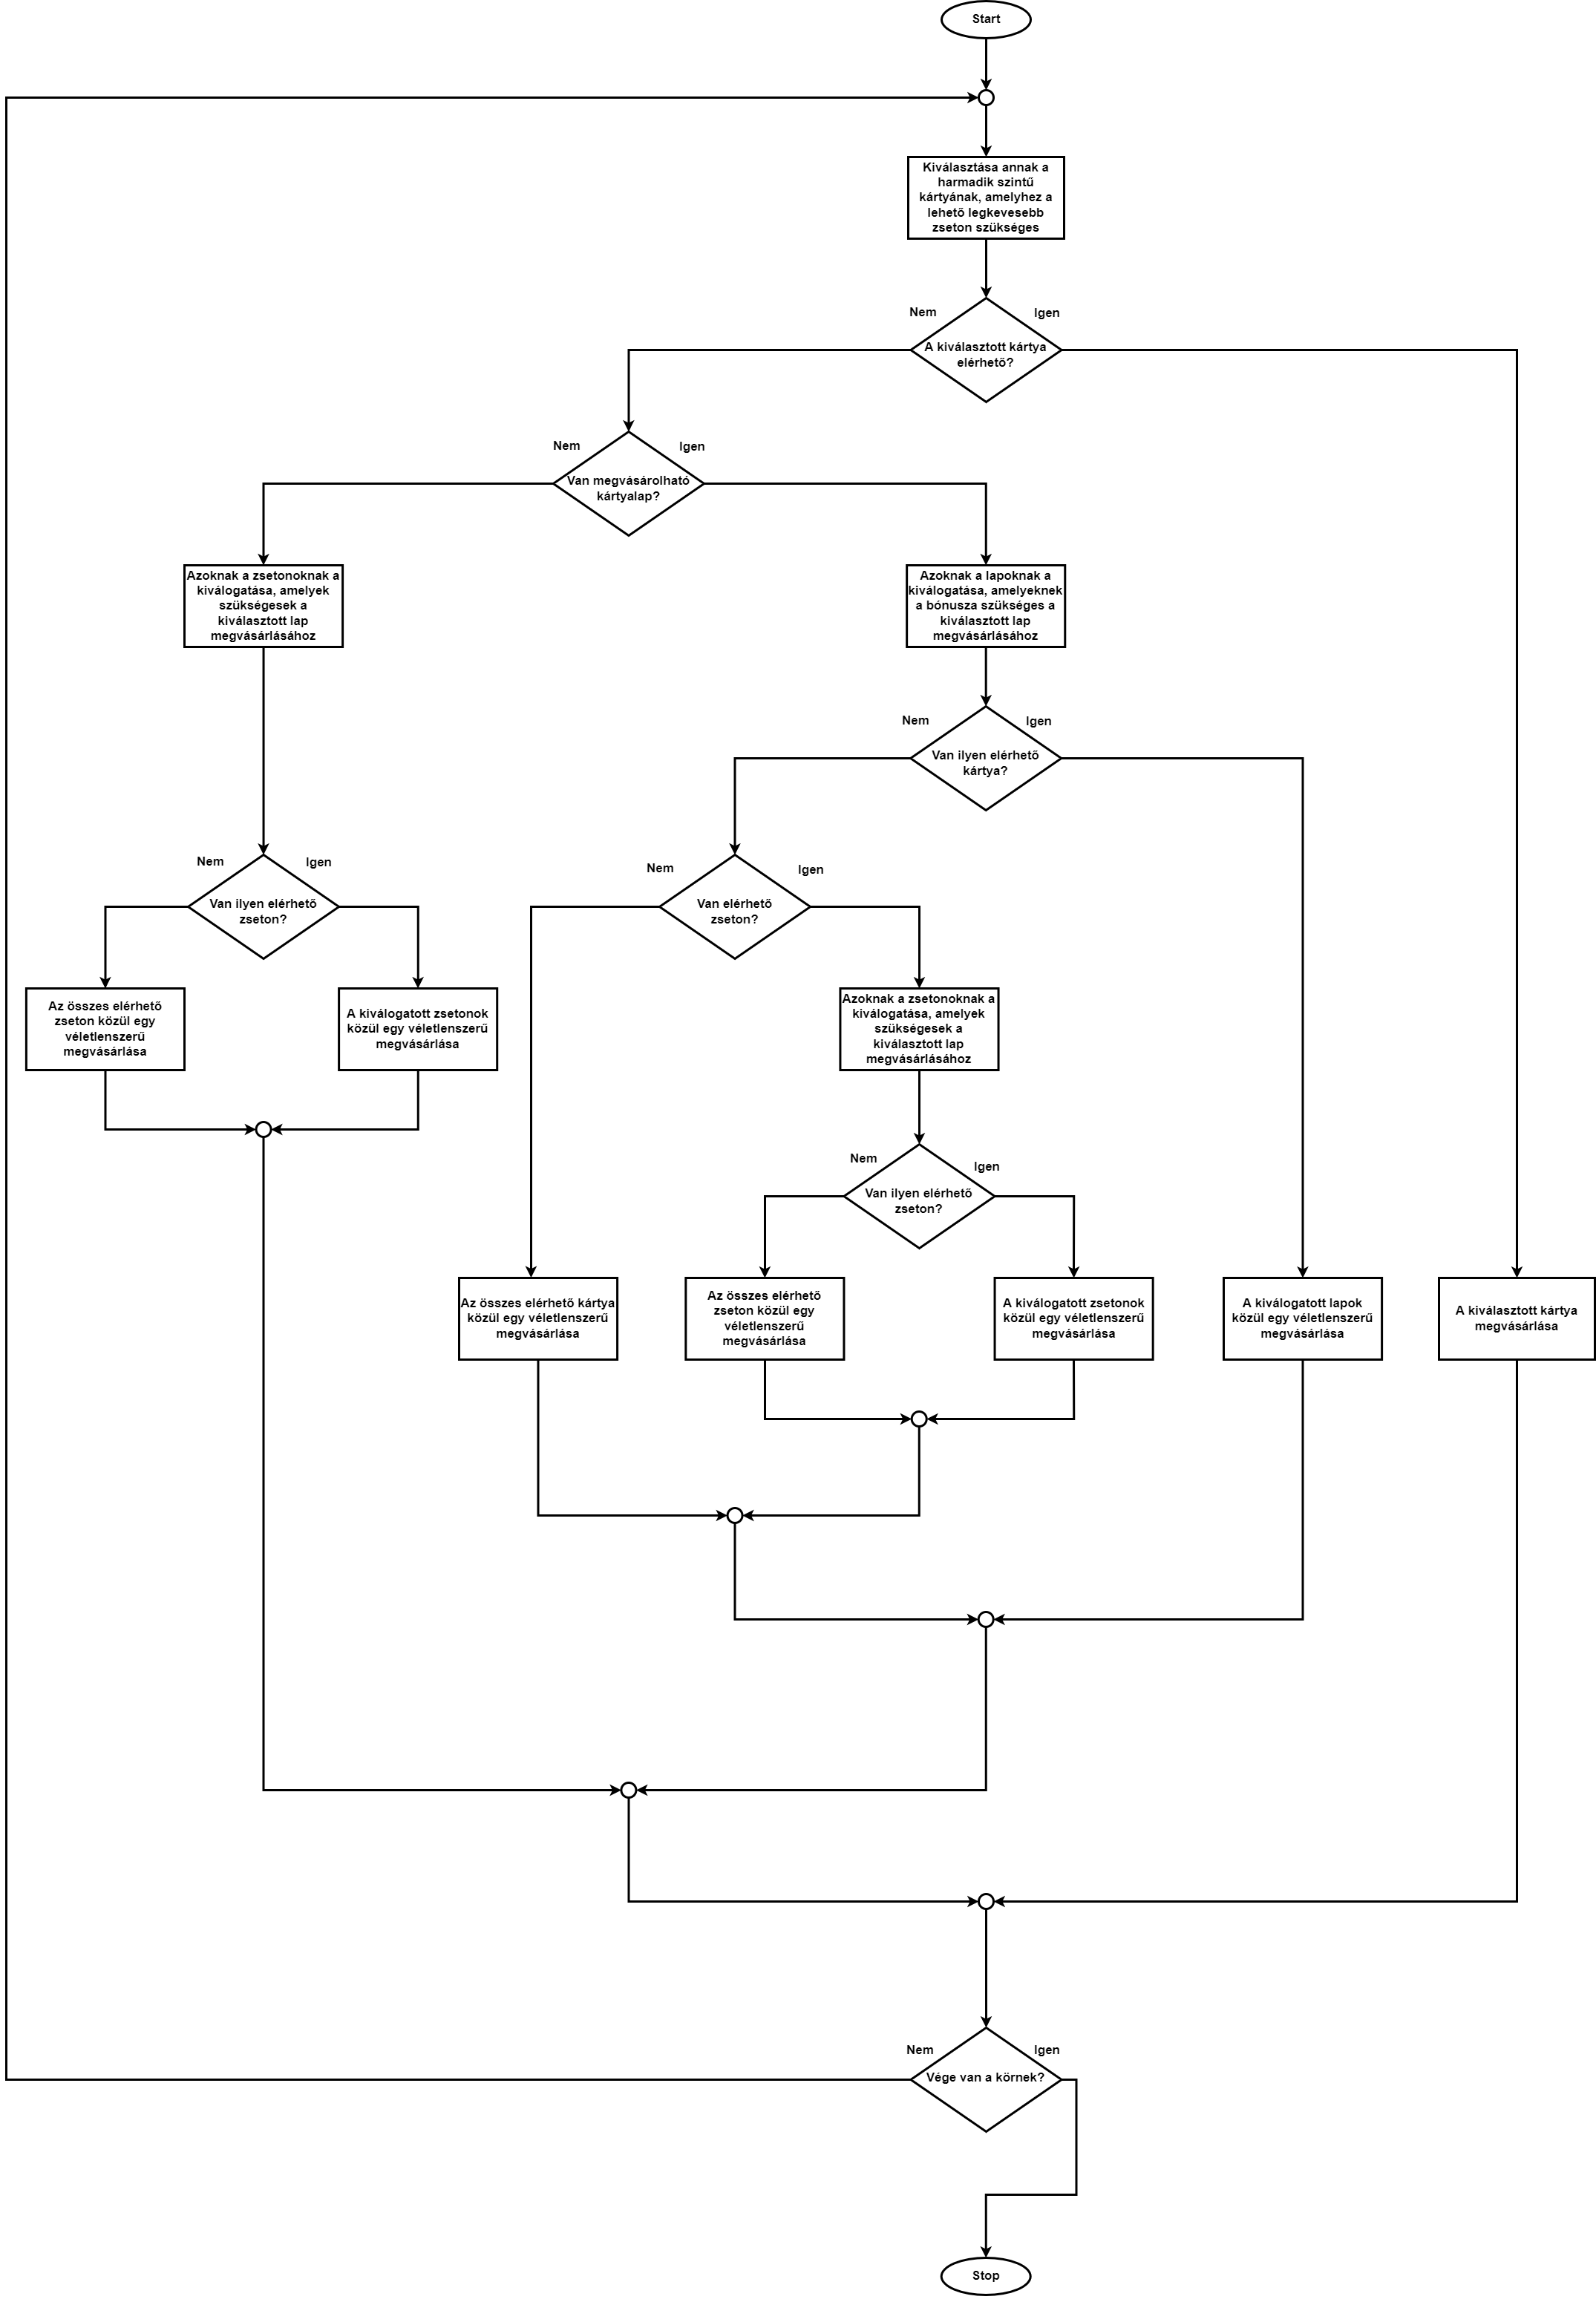
\includegraphics[scale=0.2]{images/fifthAI_flowchart.png}
\caption{Az AI5 folyamatábrája.}
\label{fig:AI5_flowchart}
\end{figure}

\clearpage

\addcontentsline{toc}{chapter}{Irodalomjegyzék}
\bibliographystyle{unsrt}
\bibliography{dolgozat.bib}

\newpage

\pagestyle{empty}

\noindent \textbf{\Large CD Használati útmutató}

\vskip 1cm

Ennek a címe lehet például \textit{A mellékelt CD tartalma} vagy \textit{Adathordozó használati útmutató} is.

Ez jellemzően csak egy fél-egy oldalas leírás.
Arra szolgál, hogy ha valaki kézhez kapja a szakdolgozathoz tartozó CD-t, akkor tudja, hogy mi hol van rajta.
Jellemzően elég csak felsorolni, hogy milyen jegyzékek vannak, és azokban mi található.
Az elkészített programok telepítéséhez, futtatásához tartozó instrukciók kerülhetnek ide.

A CD lemezre mindenképpen rá kell tenni
\begin{itemize}
\item a dolgozatot egy \texttt{dolgozat.pdf} fájl formájában,
\item a LaTeX forráskódját a dolgozatnak,
\item az elkészített programot, fontosabb futási eredményeket (például ha kép a kimenet),
\item egy útmutatót a CD használatához (ami lehet ez a fejezet külön PDF-be vagy MarkDown fájlként kimentve).
\end{itemize}


\end{document}